% =====================================================================
%  Physics and Code for Beginners -- A Guide to the Lunar-HFE Repository
%  Self-contained teaching handbook. Compile with:
%      latexmk -pdf -interaction=nonstopmode beginners_guide.tex
%  Designed to compile out-of-the-box on Overleaf (no shell-escape).
% =====================================================================
\documentclass[11pt,oneside]{article}

% ---- page geometry: generous, textbook-like margins -----------------
\usepackage[a4paper,margin=1in,headheight=14pt]{geometry}

% ---- fonts & encoding ----------------------------------------------
\usepackage[T1]{fontenc}
\usepackage[utf8]{inputenc}
\usepackage{lmodern}
\usepackage{microtype}

% ---- math ----------------------------------------------------------
\usepackage{amsmath}
\usepackage{amssymb}
\usepackage{siunitx}
\sisetup{per-mode=symbol, inter-unit-product=\ensuremath{\cdot}}

% ---- tables, graphics, lists ---------------------------------------
\usepackage{booktabs}
\usepackage{array}
\usepackage{longtable}
\usepackage{graphicx}
\graphicspath{{figures/}}
\usepackage{enumitem}
\usepackage{caption}
\captionsetup{font=small,labelfont=bf,labelsep=period}

% ---- colour palette (matches the generated figures) ----------------
\usepackage{xcolor}
\definecolor{coral}{HTML}{B85B3A}
\definecolor{teal}{HTML}{2A6478}
\definecolor{forest}{HTML}{3D6E4A}
\definecolor{plum}{HTML}{5A4A6A}
\definecolor{char}{HTML}{2A2520}
\definecolor{dim}{HTML}{6E6862}
\definecolor{paper}{HTML}{FAF7F2}
\definecolor{softgrey}{HTML}{E8E5E0}
\definecolor{codebg}{HTML}{F6F3EE}

% ---- callout boxes --------------------------------------------------
\usepackage[most]{tcolorbox}
\tcbuselibrary{skins,breakable}

\newtcolorbox{plainenglish}[1][]{%
  enhanced, breakable, colback=teal!6, colframe=teal,
  boxrule=0.6pt, arc=2pt, left=8pt, right=8pt, top=6pt, bottom=6pt,
  fonttitle=\bfseries, coltitle=teal,
  title={In plain English}, #1}

\newtcolorbox{analogy}[1][]{%
  enhanced, breakable, colback=forest!6, colframe=forest,
  boxrule=0.6pt, arc=2pt, left=8pt, right=8pt, top=6pt, bottom=6pt,
  fonttitle=\bfseries, coltitle=forest,
  title={Analogy}, #1}

\newtcolorbox{keyidea}[1][]{%
  enhanced, breakable, colback=coral!7, colframe=coral,
  boxrule=0.8pt, arc=2pt, left=8pt, right=8pt, top=6pt, bottom=6pt,
  fonttitle=\bfseries, coltitle=coral,
  title={Key idea}, #1}

\newtcolorbox{tryit}[1][]{%
  enhanced, breakable, colback=plum!6, colframe=plum,
  boxrule=0.6pt, arc=2pt, left=8pt, right=8pt, top=6pt, bottom=6pt,
  fonttitle=\bfseries, coltitle=plum,
  title={Try it yourself}, #1}

\newtcolorbox{headsup}[1][]{%
  enhanced, breakable, colback=dim!8, colframe=dim,
  boxrule=0.6pt, arc=2pt, left=8pt, right=8pt, top=6pt, bottom=6pt,
  fonttitle=\bfseries, coltitle=dim,
  title={Heads-up}, #1}

% ---- code listings (no shell-escape needed) ------------------------
\usepackage{listings}
\lstdefinestyle{pystyle}{%
  language=Python,
  backgroundcolor=\color{codebg},
  basicstyle=\ttfamily\footnotesize\color{char},
  keywordstyle=\color{teal}\bfseries,
  commentstyle=\color{forest}\itshape,
  stringstyle=\color{coral},
  numberstyle=\tiny\color{dim},
  numbers=left, numbersep=8pt,
  showstringspaces=false,
  breaklines=true, breakatwhitespace=true,
  frame=single, rulecolor=\color{softgrey},
  framesep=6pt, xleftmargin=14pt, xrightmargin=4pt,
  tabsize=4, columns=fullflexible, keepspaces=true,
  literate={~}{{\textasciitilde}}1
}
\lstdefinestyle{shellstyle}{%
  language=bash,
  backgroundcolor=\color{codebg},
  basicstyle=\ttfamily\footnotesize\color{char},
  keywordstyle=\color{teal}\bfseries,
  commentstyle=\color{dim}\itshape,
  showstringspaces=false,
  breaklines=true,
  frame=single, rulecolor=\color{softgrey},
  framesep=6pt, xleftmargin=8pt, xrightmargin=4pt,
  columns=fullflexible, keepspaces=true,
  literate={~}{{\textasciitilde}}1
}
\lstset{style=pystyle}

% ---- TikZ -----------------------------------------------------------
\usepackage{tikz}
\usetikzlibrary{arrows.meta,positioning,shapes.geometric,calc,fit,backgrounds,decorations.pathreplacing}

% ---- hyperref (load near last) -------------------------------------
\usepackage{hyperref}
\hypersetup{%
  colorlinks=true, linkcolor=teal, urlcolor=coral, citecolor=plum,
  pdftitle={Physics and Code for Beginners: A Guide to the Lunar-HFE Repository},
  pdfauthor={Lunar-HFE project}, bookmarksnumbered=true}

% ---- handy macros ---------------------------------------------------
\newcommand{\Kd}{\ensuremath{K_d}}
\newcommand{\Kdstar}{\ensuremath{K_d^{*}}}
\newcommand{\Ks}{\ensuremath{K_s}}
\newcommand{\Qb}{\ensuremath{Q_b}}
\newcommand{\code}[1]{\texttt{\small #1}}
\newcommand{\file}[1]{\texttt{\small #1}}
\newcommand{\mwmk}{\unit{mW.m^{-1}.K^{-1}}}

% =====================================================================
\begin{document}

% ---------- TITLE PAGE ----------
\begin{titlepage}
\centering
\vspace*{2.2cm}
{\color{dim}\large A hands-on companion to the Lunar-HFE research code}\\[1.6cm]
{\color{char}\Huge\bfseries Physics and Code\\[0.35cm] for Beginners}\\[0.8cm]
{\color{coral}\LARGE Measuring how the Moon's soil conducts heat}\\[2.0cm]

\begin{tcolorbox}[enhanced, width=0.82\textwidth, colback=paper,
  colframe=teal, boxrule=0.8pt, arc=3pt, halign=flush left]
\textbf{Who this is for.} You --- someone who is smart and motivated but has
\emph{no prior background} in coding, numerical methods, or heat-transfer
physics, and who wants to understand \emph{this specific project} from the
ground up.\\[4pt]
\textbf{The whole project in one sentence.} We take the only two sets of
underground temperature measurements ever made on the Moon (Apollo~15 and~17),
build a small physics simulator of how heat moves through Moon soil, and tune
one number --- the deep thermal conductivity \Kd{} --- until the simulator
matches the real measurements at each site.
\end{tcolorbox}

\vfill
{\color{dim}\small Generated teaching handbook \,\textbullet\, build the PDF with
\texttt{latexmk -pdf beginners\_guide.tex}}\\[2pt]
{\color{dim}\small Headline result: \Kdstar{}~$=$~\num{4.58}~\mwmk{} (Apollo~15),
\num{8.12}~\mwmk{} (Apollo~17).}
\vspace*{1.2cm}
\end{titlepage}

% ---------- TABLE OF CONTENTS ----------
\tableofcontents
\listoffigures
\clearpage

% ---------- HOW TO READ ----------
\section*{How to read this guide}
\addcontentsline{toc}{section}{How to read this guide}
Read it top to bottom, once, slowly. Each section builds on the one before.
Wherever you see a file path like \file{lunar/solver.py} or a function name
like \code{solve\_periodic\_equilibrium}, that is a \emph{real thing} in the
repository you can open and look at. The guide is the map; the code is the
territory. The coloured boxes are signposts:

\begin{itemize}[leftmargin=1.4em,itemsep=2pt]
  \item \textcolor{teal}{\textbf{In plain English}} --- the jargon-free version.
  \item \textcolor{forest}{\textbf{Analogy}} --- an everyday picture to lean on.
  \item \textcolor{coral}{\textbf{Key idea}} --- the one thing to remember.
  \item \textcolor{plum}{\textbf{Try it yourself}} --- a small action at the keyboard.
  \item \textcolor{dim}{\textbf{Heads-up}} --- a subtlety or common confusion.
\end{itemize}
\clearpage

% ---------- SECTIONS ----------
\section{The big picture: what question does this repo answer, and why care?}
\label{sec:bigpicture}

\subsection{The scientific question in one breath}
\label{sec:question}

How well does the loose, dusty soil on the Moon (called \textbf{regolith})
conduct heat, about a metre below the surface, \emph{at two specific places} ---
the Apollo~15 and Apollo~17 landing sites? And is that number \emph{the same at
both sites}, or different?

The single number that captures ``how well does deep Moon soil conduct heat'' is
called \Kd{} --- the \emph{deep thermal conductivity}. This whole repository
exists to measure \Kd{} at those two sites and to ask whether they differ.

\subsection{Why this is hard, and why it matters}

\begin{itemize}[leftmargin=1.4em,itemsep=3pt]
  \item The Moon has been mapped from orbit in incredible detail. But orbiters
    only see the \textbf{surface}. To know what is happening a metre \emph{down},
    you need a thermometer \emph{in the ground}.
  \item Thermometers have been buried in the Moon \textbf{exactly twice in
    history}: during Apollo~15 (1971) and Apollo~17 (1972). Astronauts drilled
    holes and dropped temperature probes down them. This was the
    \textbf{Heat-Flow Experiment (HFE)}. The instruments radioed back
    temperatures from 1971 to 1977.
  \item That 1971--1977 record is therefore \emph{the only direct measurement of
    metre-scale lunar soil conductivity that exists}. Everything else is an
    educated guess extrapolated from surface data.
  \item Current models (notably the widely used \textbf{Hayne et al.\ 2017}
    model) apply a \textbf{single conductivity value to the entire Moon}. This
    project asks: is one global number actually good enough, or do different
    places genuinely differ?
\end{itemize}

\begin{plainenglish}
We have two underground thermometers' worth of data, ever, from the whole Moon.
This project squeezes that scarce data as hard as it can to answer one sharp
question: does deep Moon soil conduct heat the same everywhere, or not?
\end{plainenglish}

\paragraph{Why anyone cares.}
\begin{itemize}[leftmargin=1.4em,itemsep=3pt]
  \item Future missions want to detect \textbf{water ice} trapped below the
    lunar surface. Whether ice stays frozen or sublimates away depends on the
    \textbf{temperature profile underground}, which depends directly on \Kd{}.
  \item An upcoming terahertz mission (\textbf{TSUKIMI}) will try to ``see'' into
    the regolith from orbit. To interpret what it sees, it needs the underground
    temperature-versus-depth curve $T(z)$ as a boundary condition --- and that
    curve is set by \Kd{}.
  \item More fundamentally: if ``one number for the whole Moon'' is wrong, every
    model built on it inherits the error.
\end{itemize}

\subsection{The headline result (the answer)}
\label{sec:headline}

After all the modelling and statistics, this is what the repository finds (these
exact numbers are committed in \file{output/kd\_retrieval\_results.json} and
quoted in the paper abstract).

\begin{table}[h]
\centering
\caption{The retrieved deep conductivity at each Apollo site.}
\label{tab:headline}
\begin{tabular}{lcc}
\toprule
\textbf{Site} & \textbf{Retrieved \Kdstar} & \textbf{Units} \\
\midrule
Apollo 15 & \textbf{4.58} \;(\textbf{+1.33} / $-$0.28) & \mwmk \\
Apollo 17 & \textbf{8.12} \;(\textbf{+0.49} / $-$0.61) & \mwmk \\
\bottomrule
\end{tabular}
\end{table}

\begin{itemize}[leftmargin=1.4em,itemsep=3pt]
  \item The little $*$ in \Kdstar{} means ``the best-fit value'' (the star is the
    retrieved estimate).
  \item The units \mwmk{} are milliwatts per metre per kelvin --- a measure of
    conductivity (\autoref{sec:conductivity} explains what conductivity units
    mean). For scale, the ``one global value'' everyone used before is
    \Kd{}~$=$~\num{3.4} in the same units, window glass is ${\sim}1000$, and
    copper is ${\sim}\num{4e8}$. Lunar regolith is an \emph{extraordinary}
    insulator.
  \item The \textbf{inter-site contrast} (the difference, A17~$-$~A15) is
    ${\approx}\,$\num{3.3}~\mwmk{}, with a 95\% confidence interval of roughly
    $[0.4, 4.6]$ that \textbf{excludes zero} ($p \approx 0.01$). In plain terms:
    the two sites really do appear to differ --- Apollo~17 soil conducts heat
    noticeably better than Apollo~15 soil --- by roughly a factor of~1.8.
\end{itemize}

\begin{keyidea}
The two sites are different. Apollo~17 deep soil conducts heat about
\textbf{1.8 times better} than Apollo~15 deep soil. That difference, established
from the only underground data that exist, is the scientific contribution of the
whole project. The rest of this guide explains \emph{how} the repository gets
there.
\end{keyidea}

\section{Notation reference --- every symbol used in this project}
\label{sec:notation}

This section is a \textbf{complete symbol map}. Keep it open while reading the
physics sections or the code. Symbols are grouped by topic; each entry gives the
meaning, typical units, and where it appears in the repository.

\subsection{Coordinates, time, and indexing}

\begin{longtable}{@{}p{0.14\linewidth} p{0.22\linewidth} p{0.18\linewidth} p{0.38\linewidth}@{}}
\toprule
Symbol & Meaning & Units & Where in code / paper \\
\midrule
\endhead
$z$ & Depth, positive \textbf{downward} from the regolith surface & \si{m} &
  \code{grid.z\_mid}, paper $z=0$ at surface \\
$t$ & Time within one lunation cycle & \si{s} &
  \code{PixelInputs.t}, hourly steps in production \\
$T(z,t)$ & Temperature at depth $z$ and time $t$ & \si{K} &
  \code{PixelOutputs.T[i,k]} \\
$T_s(t)$ & \textbf{Skin} (surface) temperature & \si{K} &
  \code{PixelOutputs.T\_surface}, solved by Newton each step \\
$\langle T\rangle(z)$ & Cycle-\textbf{mean} (time-averaged) temperature at depth $z$ &
  \si{K} & \code{EquilibriumResult.T\_mean}, ``annual mean'' in paper \\
$\partial T/\partial t$ & Rate of temperature change in time & \si{K/s} &
  discretised as $(T^{n+1}-T^n)/\Delta t$ \\
$\partial T/\partial z$ & Temperature gradient with depth & \si{K/m} &
  \code{np.gradient}, Fourier flux \\
$i$, $k$ & Grid index (depth), time index & --- &
  cell $i$, timestep $k$ in \code{PixelOutputs.T[i,k]} \\
\midrule
\endhead
\bottomrule
\end{longtable}

\subsection{Heat, flux, and energy}

\begin{longtable}{@{}p{0.14\linewidth} p{0.22\linewidth} p{0.18\linewidth} p{0.38\linewidth}@{}}
\toprule
Symbol & Meaning & Units & Where \\
\midrule
\endhead
$q$ & \textbf{Heat flux} --- thermal power crossing a horizontal plane per unit area &
  \si{W/m^2} & Fourier: $q=-K\,\partial T/\partial z$ \\
$Q_b$ & \textbf{Basal / geothermal heat flux} --- steady upward flux from the lunar
  interior at the column bottom & \si{W/m^2} &
  \code{SITES[..]['Q\_BASAL']}; A15 $=0.021$, A17 $=0.015$ \\
$u_{\mathrm{rect}}$ & \textbf{Rectified (eddy) flux} --- extra cycle-mean flux in the
  diurnal skin from $K(T)$ nonlinearity & \si{W/m^2} &
  \code{\_rectified\_flux} in \file{equilibrium.py} \\
$\rho$ & \textbf{Bulk density} of regolith & \si{kg/m^3} &
  \code{density\_hayne} \\
$c_p$ & \textbf{Specific heat} --- energy to warm \SI{1}{kg} by \SI{1}{K} &
  \si{J.kg^{-1}.K^{-1}} & \code{specific\_heat} \\
$\rho c_p$ & Volumetric heat capacity (thermal inertia per volume) &
  \si{J.m^{-3}.K^{-1}} & product \code{cap} in \code{\_step} \\
\midrule
\endhead
\bottomrule
\end{longtable}

\subsection{Thermal conductivity model (Hayne 2017)}

\begin{longtable}{@{}p{0.14\linewidth} p{0.22\linewidth} p{0.18\linewidth} p{0.38\linewidth}@{}}
\toprule
Symbol & Meaning & Units & Typical / retrieved value \\
\midrule
\endhead
$K(T,z)$ & Total effective thermal conductivity & \si{W.m^{-1}.K^{-1}} &
  \code{conductivity\_hayne} \\
$K_c(z)$ & \textbf{Structural} (contact) part of $K$ & \si{W.m^{-1}.K^{-1}} &
  rises from $K_s$ to $K_d$ with depth \\
$K_s$ & Surface contact conductivity & \si{W.m^{-1}.K^{-1}} &
  $7.4\times10^{-4}$ (\code{K\_SURFACE}) \\
\Kd & Deep contact conductivity --- \textbf{the retrieved parameter} &
  \si{W.m^{-1}.K^{-1}} & A15 \Kdstar${}=4.58$, A17 $=8.12$~\mwmk{} \\
$H$ & Compaction \textbf{scale height} for $K_c(z)$ and $\rho(z)$ & \si{m} &
  ${\sim}0.06$ (\code{H\_PARAMETER}) \\
$\chi$ & Radiative conductivity coefficient & --- &
  $2.7$ (\code{CHI\_RADIATIVE}) \\
$T_{\mathrm{ref}}$ & Reference temperature in radiative term & \si{K} &
  350 in code \\
$\rho_s$, $\rho_d$ & Surface / deep bulk density & \si{kg/m^3} &
  ${\sim}1100$ / ${\sim}1800$ \\
\midrule
\endhead
\bottomrule
\end{longtable}

\subsection{Surface radiation, albedo, and orbital forcing}

\begin{longtable}{@{}p{0.14\linewidth} p{0.22\linewidth} p{0.18\linewidth} p{0.38\linewidth}@{}}
\toprule
Symbol & Meaning & Units & Typical / code \\
\midrule
\endhead
$S_0$ & Solar constant at 1~AU (flux at top of atmosphere) & \si{W/m^2} &
  1361 (\code{S0} in \file{config.py}) \\
$F_\odot(t)$, $S(t)$ & \textbf{Insolation} --- solar irradiance on local horizontal
  surface & \si{W/m^2} & \code{insolation} array in \code{run\_with} \\
$\theta_\odot(t)$ & \textbf{Solar zenith angle} --- angle from local vertical to Sun &
  rad or \si{\degree} & idealised: $\cos\theta_\odot=\cos\phi\cos(2\pi t/P)$ \\
$\phi$ & Site \textbf{latitude} (north positive) & \si{\degree} &
  A15 $26.13^\circ$N, A17 $20.19^\circ$N \\
$P$ & Mean \textbf{synodic lunation} (Sun $\to$ Sun as seen from site) & \si{s} &
  $2\,551\,443$ (\code{T\_LUNAR}) \\
$A$ & \textbf{Bond albedo} --- fraction of sunlight reflected & --- &
  ${\sim}0.13$ per site \\
$(1-A)$ & Fraction of sunlight \textbf{absorbed} at surface & --- &
  ${\sim}0.87$ \\
$\varepsilon$ & \textbf{Emissivity} --- efficiency of thermal radiation & --- &
  0.95 \\
$\sigma$ & Stefan--Boltzmann constant & \si{W.m^{-2}.K^{-4}} &
  $5.6704\times10^{-8}$ (\code{SIGMA\_SB}) \\
$\varepsilon\sigma T_s^4$ & Outgoing thermal (infrared) radiative flux & \si{W/m^2} &
  surface energy balance \\
\midrule
\endhead
\bottomrule
\end{longtable}

\subsection{Boundary conditions and problem setup}

\begin{longtable}{@{}p{0.14\linewidth} p{0.22\linewidth} p{0.18\linewidth} p{0.38\linewidth}@{}}
\toprule
Symbol & Meaning & Where \\
\midrule
\endhead
Eq.~\eqref{eq:heat} & Interior \textbf{heat equation} (PDE) & all interior cells \\
Eq.~\eqref{eq:bc-top-teach} & \textbf{Top BC}: radiative surface energy balance &
  \code{surface\_energy\_balance\_residual} \\
Eq.~\eqref{eq:bc-bot-teach} & \textbf{Bottom BC}: prescribed basal flux $Q_b$ &
  \code{d[-1] += dt*Q\_b/cap[-1]} \\
$z_{\mathrm{max}}$ & Bottom of model column & 5~\si{m} (\code{GRID['z\_max']}) \\
$z_{\mathrm{anchor}}$ & Anchor depth for equilibrium method & 0.55~\si{m} \\
\midrule
\endhead
\bottomrule
\end{longtable}

\subsection{Skin depth, diffusivity, and diurnal damping}

\begin{longtable}{@{}p{0.14\linewidth} p{0.22\linewidth} p{0.18\linewidth} p{0.38\linewidth}@{}}
\toprule
Symbol & Meaning & Formula / value \\
\midrule
\endhead
$\alpha$ & Thermal diffusivity & $\alpha = K/(\rho c_p)$ \\
$\omega$ & Angular frequency of diurnal forcing & $\omega = 2\pi/P$ \\
$\delta$ & \textbf{Thermal skin depth} & $\delta = \sqrt{2\alpha/\omega}$; few cm \\
\midrule
\endhead
\bottomrule
\end{longtable}

\subsection{Numerical discretisation}

\begin{longtable}{@{}p{0.14\linewidth} p{0.22\linewidth} p{0.18\linewidth} p{0.38\linewidth}@{}}
\toprule
Symbol & Meaning & Production value \\
\midrule
\endhead
$\Delta z_i$, \code{dz} & Thickness of layer $i$ (geometric grid) & \SI{2}{mm} at top, grows ${\sim}8\%$/layer \\
$\Delta t$ & Timestep & \SI{1}{h} (\code{DT\_STEP}) \\
$N_z$ & Number of depth cells & ${\sim}69$ for 5~\si{m} column \\
$N_t$ & Timesteps per lunation & 709 \\
\midrule
\endhead
\bottomrule
\end{longtable}

\subsection{Retrieval, data, and statistics}

\begin{longtable}{@{}p{0.14\linewidth} p{0.22\linewidth} p{0.18\linewidth} p{0.38\linewidth}@{}}
\toprule
Symbol & Meaning & Where \\
\midrule
\endhead
\Kdstar & Retrieved deep conductivity minimising RMSE & \code{kd\_retrieval\_results.json} \\
$T_{\mathrm{eq},i}$ & Equilibrium temperature at sensor $i$ (stable window mean) &
  \code{extract\_sensor\_stability} \\
$R_i$ & Residual $T_{\mathrm{model}} - T_{\mathrm{eq}}$ at sensor $i$ & \code{run\_kd\_sweep\_extended} \\
RMSE & Root mean square error of residuals & \code{kd\_star\_from\_residuals} \\
\midrule
\endhead
\bottomrule
\end{longtable}

\begin{keyidea}
\textbf{Sign conventions used throughout.} Depth $z$ increases \textbf{downward}.
Heat flux $q$ is positive when flowing \textbf{downward} (Fourier: $q=-K\,\partial T/\partial z$).
Basal flux $Q_b$ is positive when flowing \textbf{upward} from the interior --- so at
the bottom boundary $-K\,\partial T/\partial z = Q_b$ implies $\partial T/\partial z > 0$
(warmer with depth). Temperature is always in \textbf{kelvin} (K), never Celsius, in
the solver.
\end{keyidea}

\section{Physics fundamentals, from scratch}
\label{sec:physics}

This section assumes you know nothing about heat physics. Take it slowly.

\subsection{Heat vs.\ temperature (they are not the same thing)}

\begin{itemize}[leftmargin=1.4em,itemsep=3pt]
  \item \textbf{Temperature} is \emph{how hot something is} --- a single number
    at a point, like \SI{300}{\kelvin}. It tells you the average jiggling energy
    of the atoms there.
  \item \textbf{Heat} is \emph{energy in transit} --- energy flowing from a
    hotter place to a colder place. You measure it as a \emph{rate of flow}.
\end{itemize}

\begin{analogy}
Temperature is like the \textbf{water level} in a tank; heat is like the
\textbf{water flowing} between tanks. Two tanks at the same level (same
temperature) have no flow between them, even if one is huge and one is tiny.
\end{analogy}

\textbf{Kelvin (K)} is just the temperature scale scientists use. It starts at
absolute zero (the coldest possible), so there are no negative numbers.
\SI{0}{\celsius} $=$ \SI{273.15}{\kelvin}. Lunar daytime soil-surface can hit
${\sim}\SI{390}{\kelvin}$ (scorching); lunar night can fall below
\SI{100}{\kelvin} ($-\SI{170}{\celsius}$). A metre down, it settles to a
near-constant ${\sim}\SI{250}{\kelvin}$.

\subsection{Conduction: how heat moves through a solid}

There are three ways heat travels: \textbf{conduction} (through direct contact,
atom bumping atom), \textbf{convection} (carried by a moving fluid like air or
water), and \textbf{radiation} (electromagnetic waves, like sunlight or the
warmth you feel from a fire).

The Moon has \textbf{no air and no water underground}, so inside the regolith
column there is essentially only \textbf{conduction} (plus a small radiative
effect across the tiny gaps between dust grains, which we fold into an
``effective'' conductivity --- see \autoref{sec:conductivity}). This is why the
model is ``1-D conduction.''

The basic law of conduction (\textbf{Fourier's law}) says, in words: \emph{heat
flows from hot to cold, and the rate of flow is proportional to how steep the
temperature change is, times how good a conductor the material is.} As a tiny
equation,
\begin{equation}
  q \;=\; -\,K\,\frac{\mathrm{d}T}{\mathrm{d}z},
  \label{eq:fourier}
\end{equation}
where:
\begin{itemize}[leftmargin=1.4em,itemsep=3pt]
  \item $\mathrm{d}T/\mathrm{d}z$ is the \textbf{temperature gradient}: how fast
    temperature changes as you go down ($z$ is depth). Steep gradient $\to$ fast
    flow.
  \item $K$ is the \textbf{thermal conductivity}: the material property --- high
    $K$ means heat flows easily (metal), low $K$ means it resists (styrofoam,
    lunar dust).
  \item The minus sign just means heat flows \emph{down} the gradient, from hot
    to cold.
\end{itemize}
In this repo Fourier's law literally appears as the conductive term in the
surface energy balance and in every interior step. See
\code{surface\_energy\_balance\_residual} in \file{lunar/solver.py}.

\subsection{The 1-D heat equation --- full derivation from scratch}
\label{sec:heateq}

This section answers three questions in order: (1)~what problem is the code
actually solving? (2)~where does the differential equation come from, step by
step, with no prior PDE course assumed? (3)~what do the top and bottom
boundaries mean? The final equation is the one in \file{lunar/solver.py} and
in the paper (Eq.~\eqref{eq:heat}).

\subsubsection{The problem in one sentence}

\begin{keyidea}
Given how sunlight hits the lunar surface hour by hour, and given how the soil
conducts heat at each depth, \textbf{find} the temperature $T$ at every depth
$z$ and every time $t$.
\end{keyidea}

The simulator predicts a \textbf{temperature profile through the soil column}
--- temperatures from the surface down to \SI{5}{m} --- and updates that
profile as the lunar day/night cycle rolls on. In code, the answer lives in
\code{PixelOutputs.T} from \code{solve\_pixel} in \file{lunar/solver.py}: a
2-D array of shape \code{(N\_z, N\_t)}.

\subsubsection{Picture a thin horizontal slice of soil}

Imagine the regolith as a \textbf{stack of thin horizontal pancakes}, each
between depth $z$ and $z+\Delta z$. Focus on one pancake in the middle:

\begin{verbatim}
     surface (z = 0)  <- sunlight, radiation to space
  -----------------------------------------
        warmer layer
  -----------------------------------------   <- top face (depth z)
        OUR SLICE  (thickness Delta z)
  -----------------------------------------   <- bottom face (z + Delta z)
        cooler layer
  -----------------------------------------
        ...
  -----------------------------------------
     bottom (z = 5 m)  <- steady heat from interior
\end{verbatim}

We track a column of soil \SI{1}{m} $\times$ \SI{1}{m} in footprint. The
slice has mass $\rho\,\Delta z$ per m$^2$ and thermal mass $\rho\,c_p\,\Delta z$
--- energy needed to warm it by \SI{1}{\kelvin}. The product $\rho\,c_p$ is
\textbf{thermal inertia}: dense, high-$c_p$ soil is hard to warm or cool (like a
heavy cast-iron pan).

\subsubsection{Heat flux at each face}

\textbf{Heat flux} $q$ [\unit{W.m^{-2}}] is the rate thermal energy crosses a
horizontal plane. Fourier's law (Eq.~\eqref{eq:fourier}) gives
\begin{equation}
  q(z) \;=\; -\,K(T,z)\,\frac{\partial T}{\partial z}.
\end{equation}
Heat flows from hot toward cold. For a slice between $z$ and $z+\Delta z$,
let $q_\mathrm{in}$ be flux across the top face and $q_\mathrm{out}$ across the
bottom.

\subsubsection{Energy conservation (the bookkeeping step)}

Energy is not created or destroyed in the slice:
\begin{equation}
  \underbrace{\rho\,c_p\,\Delta z\,\frac{\partial T}{\partial t}}_{\text{rate stored energy changes}}
  \;=\;
  q_\mathrm{in} - q_\mathrm{out}.
  \label{eq:slice-balance}
\end{equation}
The left side is how fast the slice warms; the right side is net heat flowing
in.

\subsubsection{From two faces to a derivative}

For a thin slice, $q_\mathrm{out} - q_\mathrm{in} \approx
(\partial q/\partial z)\,\Delta z$, so
$q_\mathrm{in} - q_\mathrm{out} \approx -(\partial q/\partial z)\,\Delta z$.
Substitute into Eq.~\eqref{eq:slice-balance} and cancel $\Delta z$:
\begin{equation}
  \rho\,c_p\,\frac{\partial T}{\partial t} \;=\; -\,\frac{\partial q}{\partial z}.
\end{equation}
Insert $q = -K\,\partial T/\partial z$:
\begin{equation}
  \rho(z)\,c_p(T)\,\frac{\partial T}{\partial t}
   \;=\; \frac{\partial}{\partial z}\!\left[\,K(T,z)\,\frac{\partial T}{\partial z}\,\right].
  \label{eq:heat}
\end{equation}
That is the \textbf{1-D heat equation} --- the single rule the whole simulator
enforces.

\begin{plainenglish}
\textbf{Why ``partial'' derivatives?} $T$ depends on \emph{both} depth $z$
\emph{and} time $t$. $\partial T/\partial t$ means ``how fast temperature at
this depth is changing right now''; $\partial T/\partial z$ means ``how steep
the profile is at this instant.'' You do not need a full PDE course to use
this --- treat them as separate rates of change.
\end{plainenglish}

\begin{plainenglish}
\textbf{Discrete version (what the computer does).} On a finite grid,
\begin{equation*}
  (\rho c_p)_i\,\frac{T_i^{n+1}-T_i^{n}}{\Delta t}
  = \text{(flux in from above)} - \text{(flux out below)}.
\end{equation*}
Crank--Nicolson (\autoref{sec:cn}) rearranges this so $\Delta t =
\SI{1}{h}$ is stable. Inside \code{\_step} in \file{lunar/solver.py}:
\code{cap\_i * dT\_i/dt = flux\_right(i) - flux\_left(i)}.
\end{plainenglish}

\subsubsection{Reading the final equation, term by term}

\begin{center}
\small
\begin{tabular}{@{}lll@{}}
\toprule
Piece & Plain English & Code \\
\midrule
$T(z,t)$ & Temperature at depth $z$, time $t$ & \code{PixelOutputs.T[i,k]} \\
$\partial T/\partial t$ & Warming/cooling rate & finite difference over $\Delta t$ \\
$\rho(z)$, $c_p(T)$ & Density, specific heat & \code{rho\_func}, \code{cp\_func} \\
$\rho\,c_p$ & Thermal inertia & \code{cap} in \code{\_step} \\
$K(T,z)$ & Conductivity & \code{K\_func} \\
$K\,\partial T/\partial z$ & Heat flux (Fourier) & face fluxes in \code{\_step} \\
$\partial/\partial z[\cdots]$ & Net flux in minus out & difference of face fluxes \\
\bottomrule
\end{tabular}
\end{center}

\textbf{Left side} = storage; \textbf{right side} = net conduction from
neighbours. When $K$ varies with $z$ or $T$, it stays \emph{inside} the
$\partial/\partial z$ --- the same gradient can carry different flux where
conductivity changes.

\subsubsection{The two boundaries (summary)}

The PDE needs two boundary conditions. \textbf{\autoref{sec:bc-full}} derives
them from scratch; \textbf{\autoref{sec:orbit-top-bc}} adds orbital geometry,
insolation diagrams, and the surface energy-balance figure.
both from scratch and explains their connection to the interior equation and
to \file{lunar/solver.py}. In brief: top radiative balance
(Eq.~\eqref{eq:bc-top-teach}); bottom geothermal flux
(Eq.~\eqref{eq:bc-bot-teach}).

\subsubsection{What ``solving'' means in this repository}

The simulator solves an \textbf{initial-boundary-value problem}:
\begin{enumerate}[leftmargin=1.5em,itemsep=3pt]
  \item \textbf{PDE} (interior): Eq.~\eqref{eq:heat}.
  \item \textbf{Top BC} (each timestep): Eq.~\eqref{eq:bc-top-teach}.
  \item \textbf{Bottom BC}: Eq.~\eqref{eq:bc-bot-teach}.
  \item \textbf{Initial condition}: starting profile $T(z,t{=}0)$ --- the
    equilibrium driver (\autoref{sec:anchor}) removes dependence on the guess.
\end{enumerate}

\textbf{One timestep} in \code{solve\_pixel}: evaluate $K,\rho,c_p$; assemble
Crank--Nicolson; Newton solve for $T_s$; tridiagonal solve (\code{\_thomas}) for
interior cells; advance by $\Delta t$. Repeat $\sim$709 steps per lunation.

\begin{headsup}
\textbf{Sanity checks.} (i)~Flat $T$ $\Rightarrow$ zero flux $\Rightarrow$
$\partial T/\partial t = 0$. (ii)~Steady state with bottom heat $\Rightarrow$
$\mathrm{d}\langle T\rangle/\mathrm{d}z = Q_b/K$ (geothermal gradient).
(iii)~Larger $K$ $\Rightarrow$ deeper diurnal damping (larger skin depth).
These are exactly what the code exhibits.
\end{headsup}

``1-D'' means we only track depth ($z$), ignoring sideways variation --- valid
over the small patch around a borehole.

\subsection{The three soil properties --- what they mean and why the heat equation needs them}
\label{sec:properties}

\subsubsection{Thermal capacity: why $\rho\,c_p$ sits on the left}

When you warm soil, you store \textbf{internal energy}. For a slice of thickness
$\Delta z$ and footprint \SI{1}{m^2}:
\[
  \text{mass} = \rho\,\Delta z \quad (\si{kg/m^2}), \qquad
  \text{energy to warm by \SI{1}{\kelvin}} = \rho\,c_p\,\Delta z \quad (\si{J/m^2}).
\]
So $\rho\,c_p$ is \textbf{volumetric heat capacity} (\si{J.m^{-3}.K^{-1}}). Dividing
the energy-balance rate by this capacity gives the warming rate --- exactly why
$\rho$ and $c_p$ multiply on the \textbf{left} of Eq.~\eqref{eq:heat}.

\begin{center}
\small
\begin{tabular}{@{}llll@{}}
\toprule
Symbol & Name & Units & Code \\
\midrule
$\rho(z)$ & Density & \si{kg/m^3} & \code{density\_hayne} \\
$c_p(T)$ & Specific heat & \si{J.kg^{-1}.K^{-1}} & \code{specific\_heat} \\
$\rho c_p$ & Volumetric heat capacity & \si{J.m^{-3}.K^{-1}} & \code{cap} in \code{\_step} \\
$K(T,z)$ & Conductivity & \si{W.m^{-1}.K^{-1}} & \code{conductivity\_hayne} \\
\bottomrule
\end{tabular}
\end{center}

\begin{analogy}
$\rho\,c_p$ is the soil's \textbf{thermal mass} (hard to change temperature).
$K$ is its \textbf{conductance} (how easily heat travels through).
\end{analogy}

All three are evaluated at every grid cell from \file{lunar/properties.py}.

\subsection{Thermal conductivity \texorpdfstring{$K(T,z)$}{K(T,z)} --- full physical picture}
\label{sec:conductivity}

\Kd{} --- the quantity this project retrieves --- lives inside the conductivity
formula. Two channels carry heat in vacuum regolith:

\begin{enumerate}[leftmargin=1.5em,itemsep=3pt]
  \item \textbf{Contact conduction} --- grain-to-grain; weak when fluffy.
  \item \textbf{Radiative conduction across vacuum gaps} --- grows with $T^3$.
\end{enumerate}

Hayne splits these explicitly:
\[
  K(T,z) = \underbrace{K_c(z)}_{\text{structural}} \times
           \underbrace{\bigl[1 + \chi\,(T/350)^3\bigr]}_{\text{radiative boost}}.
\]

\subsubsection{Structural part $K_c(z)$ --- compaction with depth}
\begin{equation}
  K_c(z) = K_d - (K_d - K_s)\,e^{-z/H}.
  \label{eq:kc}
\end{equation}
At $z{=}0$: $K_c{=}K_s$ (fluffy surface, ${\sim}0.74$~\mwmk). Deep down:
$K_c\to K_d$ (the unknown we fit). The scale height $H\sim\SI{6}{cm}$ sets how
fast the transition happens; at $z{=}H$ the rise is ${\sim}63\%$ complete.

\subsubsection{Radiative boost --- why $T^3$?}
Across a vacuum gap, net radiative flux $\propto T_1^4 - T_2^4 \approx 4T^3\Delta T$
for small $\Delta T$. Hayne folds this into:
\begin{equation}
  K(T,z) = K_c(z)\,\bigl[\,1 + \chi\,(T/350)^3\,\bigr].
  \label{eq:krad}
\end{equation}
At $T\approx\SI{250}{\kelvin}$ the factor is ${\sim}2$ --- radiation roughly
\textbf{doubles} effective $K$. \textbf{Not optional} (known bug if omitted).

\subsubsection{Density and specific heat}
Density compacts with the same exponential form (Hayne Eq.~5):
$\rho(z)=\rho_d-(\rho_d-\rho_s)e^{-z/H}$.
Specific heat $c_p(T)$ is a 4th-order polynomial (\code{specific\_heat}); it sets
thermal inertia but is not the retrieval's free parameter.

So \Kd{} is one knob in a fixed published shape; the retrieval freezes $K_s$, $H$,
$\chi$, and slides only \Kd{} until the model matches Apollo data.

\begin{lstlisting}[caption={Cited conductivity constants in \file{lunar/constants.py}.}]
# Surface contact conductivity [W m^-1 K^-1] -- Hayne et al. (2017) Table 2.
K_SURFACE: float = 7.4e-4
# Deep contact conductivity [W m^-1 K^-1] -- Hayne et al. (2017) Table 2.
K_DEEP: float = 3.4e-3
# Radiative conductivity coefficient chi [dimensionless] -- Hayne et al. (2017).
CHI_RADIATIVE: float = 2.7
\end{lstlisting}

\begin{headsup}
\textbf{Units.} Conductivity is in \unit{W.m^{-1}.K^{-1}} (watts per metre per
kelvin). $3.4\times10^{-3}$~\unit{W.m^{-1}.K^{-1}} $=$ \num{3.4}~\mwmk{} --- the
paper quotes milliwatts (mW) because the numbers are tiny. \SI{1}{W} $=$
\SI{1000}{mW}. So the committed \Kdstar{}~$=4.58\times10^{-3}$ in the JSON prints
as \num{4.58}~\mwmk{}.
\end{headsup}

\begin{figure}[h]
\centering
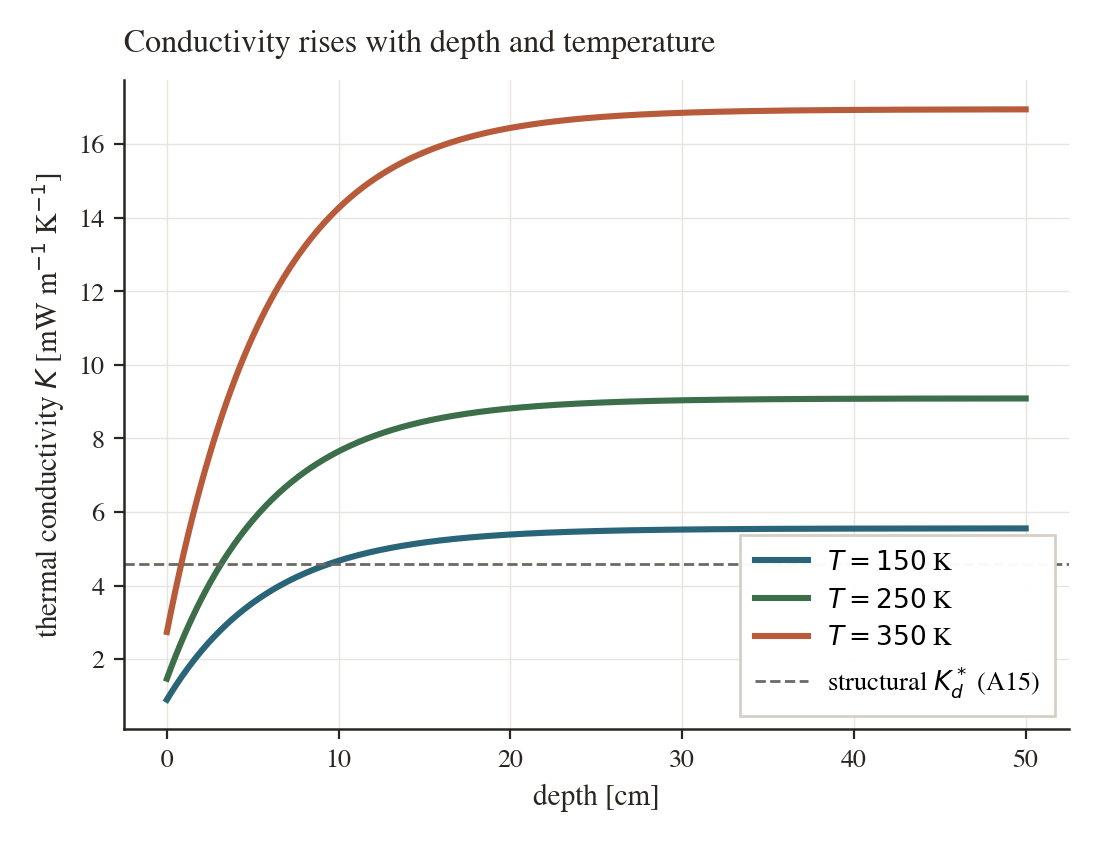
\includegraphics[width=0.78\textwidth]{fig_conductivity.png}
\caption[Conductivity rises with depth and temperature]{The Hayne $K(T,z)$ law,
Eqs.~\eqref{eq:kc}--\eqref{eq:krad}, at the Apollo~15 \Kdstar. \textbf{What to
notice:} each curve climbs steeply over the first few centimetres --- that is the
structural rise from fluffy surface ($K_s$) toward the deep value $K_d$ governed
by the scale height $H$. The three curves (cold to hot) are spread apart by the
radiative $T^3$ boost: hotter soil conducts \emph{better} even at the same depth.
\textbf{Why it matters:} the single deep number we retrieve, \Kdstar, is the
plateau these curves are climbing toward.}
\label{fig:conductivity}
\end{figure}

\subsection{The thermal skin and skin depth --- full derivation}
\label{sec:skin}

\subsubsection{Thermal diffusivity}
\[
  \alpha = \frac{K}{\rho\,c_p} \quad [\si{m^2/s}].
\]
Dividing the heat equation by $\rho c_p$ (constant properties):
$\partial T/\partial t = \alpha\,\partial^2 T/\partial z^2$ --- a diffusion equation.

\subsubsection{The decaying thermal wave}
For sinusoidal surface forcing $T(0,t)=T_{\mathrm{mean}}+A_s\cos(\omega t)$:
\[
  T(z,t) = T_{\mathrm{mean}} + A_s\,e^{-z/\delta}\cos(\omega t - z/\delta).
\]
At $z=\delta$ the amplitude is $A_s/e\approx 0.37A_s$.

\subsubsection{Deriving the skin depth}
Substituting into the diffusion equation gives
\begin{equation}
  \delta = \sqrt{\frac{2\alpha}{\omega}}.
  \label{eq:skin}
\end{equation}
Larger $\alpha$ $\Rightarrow$ deeper skin; larger $\omega$ $\Rightarrow$ shallower
skin. For the Moon, $\delta\sim\SI{6}{cm}$.

Apollo sensors at \SI{0.8}{m}--\SI{2.4}{m} sit \textbf{10--40$\times$ deeper}
than $\delta$ --- below the diurnal noise, in the quiet zone set by the geothermal
gradient. This underpins \code{MIN\_DEPTH\_CM = 80} and the Anchor Point Method.

\begin{figure}[h]
\centering
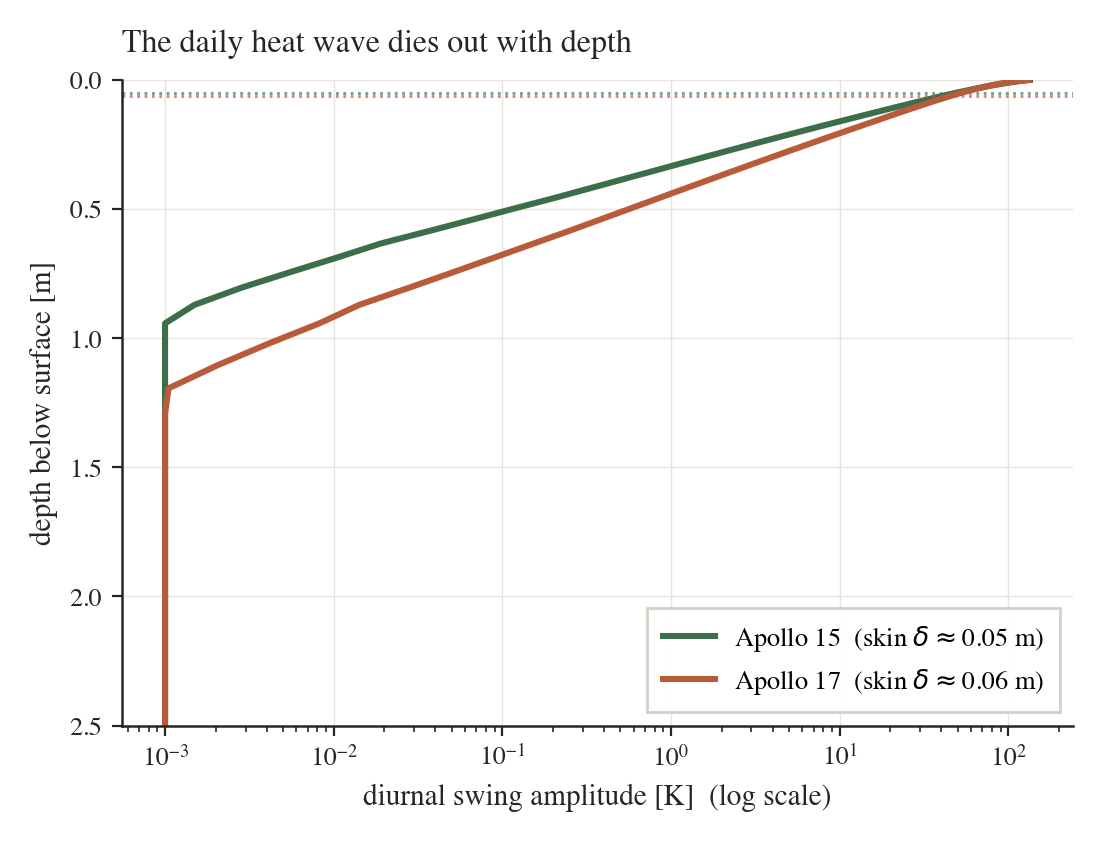
\includegraphics[width=0.78\textwidth]{fig_skin_depth.png}
\caption[The daily heat wave dies out with depth]{The size of the day/night
temperature swing as you go down, for both sites (note the \emph{logarithmic}
horizontal axis). \textbf{What to notice:} the swing starts at ${\sim}100$~K at
the surface and collapses by a factor of a thousand within about a metre --- the
dotted line marks the $1/e$ skin depth $\delta$, only a few centimetres. Below
that the curve plunges to essentially nothing. \textbf{Why it matters:} the
Apollo sensors used for the fit all sit well below this skin, in the quiet zone
where temperature is set purely by the deep heat flow.}
\label{fig:skin}
\end{figure}

\subsection{Radiation, sunlight, and the geothermal gradient --- full picture}
\label{sec:boundaries}

\subsubsection{Stefan--Boltzmann: why $T^4$?}
Every surface emits radiation $q_{\mathrm{rad}}=\varepsilon\sigma T^4$. A slightly
hotter surface radiates vastly more ($2\times$ temperature $\Rightarrow 16\times$
power). This makes the surface balance non-linear (Newton solve, \autoref{sec:newton}).

\subsubsection{Surface energy balance}
\begin{equation}
  \underbrace{(1-A)\,S(t)}_{\text{absorbed}}
   \;-\; \underbrace{\varepsilon\sigma T_s^4}_{\text{radiated}}
   \;-\; \underbrace{q_{\mathrm{cond}}(0)}_{\text{into soil}}
   \;=\; 0.
  \label{eq:surface}
\end{equation}
Implemented in \code{surface\_energy\_balance\_residual} (\file{lunar/solver.py}).

\subsubsection{Insolation model}
\[
  S(t) = S_0\cos(\mathrm{lat})\,\max\!\bigl(0,\cos(2\pi t/T_{\mathrm{lunation}})\bigr).
\]
Built in \code{run\_with}. Idealised diurnal cosine; neglected terms are bounded in
the paper.

\subsubsection{Geothermal gradient --- full derivation}
Bottom BC: $-K\,\partial T/\partial z|_{\mathrm{bottom}} = Q_b$.
Time-average the heat equation in periodic steady state ($\partial\langle T\rangle/\partial t=0$):
\[
  \frac{\partial}{\partial z}\!\Bigl[K\,\frac{\partial\langle T\rangle}{\partial z}\Bigr]=0
  \quad\Rightarrow\quad K\,\frac{\mathrm{d}\langle T\rangle}{\mathrm{d}z}=\mathrm{const}=Q_b.
\]
Hence
\begin{equation}
  \frac{\mathrm{d}\langle T\rangle}{\mathrm{d}z} = \frac{Q_b}{K}.
  \label{eq:geotherm}
\end{equation}
Larger $Q_b$ or smaller $K$ $\Rightarrow$ steeper rising mean profile. Example:
$Q_b=0.021$~\si{W/m^2}, $K_d\approx 0.0046$~\si{W/m/K} $\Rightarrow$
gradient $\approx\SI{4.6}{K/m}$.

This \Qb{} matters for the retrieval: deep $T$ depends on the \textbf{ratio}
$Q_b/K_d$ --- the \textbf{\Kd--\Qb{} degeneracy} (\autoref{sec:degeneracy}).

\begin{figure}[h]
\centering
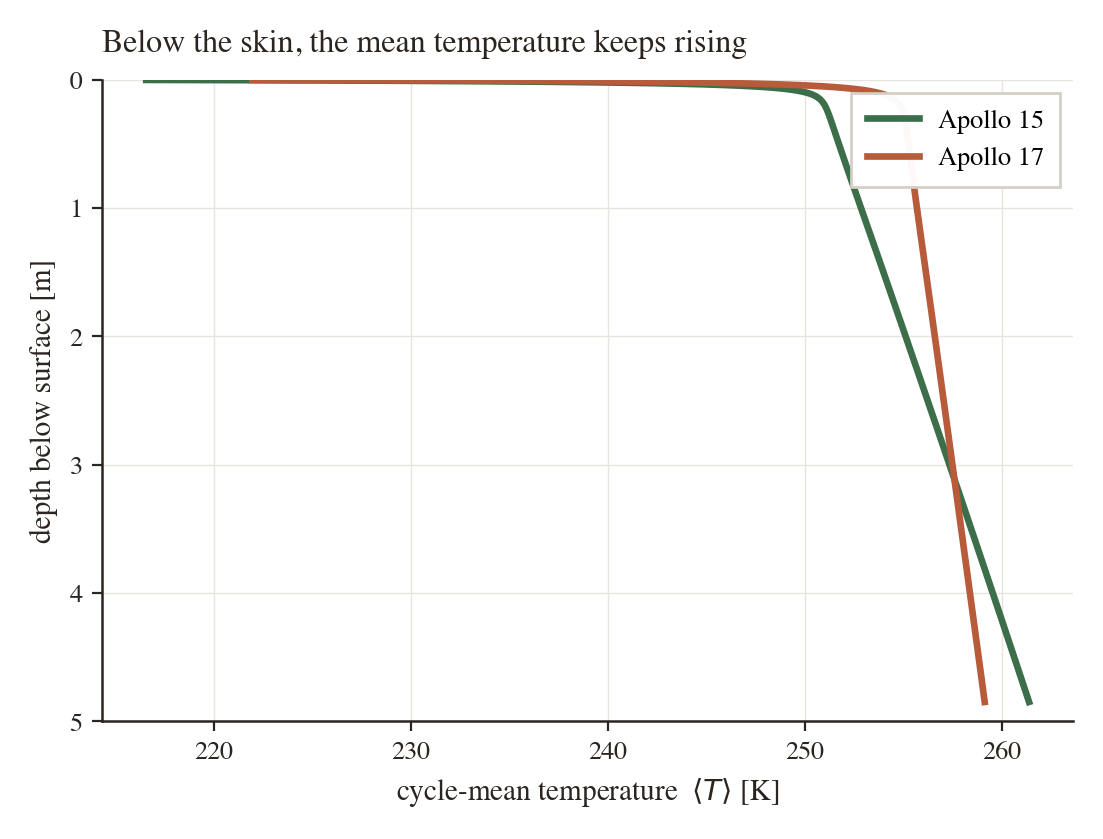
\includegraphics[width=0.78\textwidth]{fig_mean_profile.png}
\caption[Below the skin the mean temperature keeps rising]{The cycle-averaged
temperature $\langle T\rangle$ versus depth for both sites, from the certified
equilibrium solver. \textbf{What to notice:} below ${\sim}1$~m the curve becomes
a straight, \emph{tilted} line --- it does not flatten out. That tilt is the
geothermal gradient $Q_b/K$ of Eq.~\eqref{eq:geotherm}. \textbf{Why it matters:}
the deep slope encodes the ratio $Q_b/K_d$; reading the Apollo temperatures
against this line is exactly how the project pins down \Kd.}
\label{fig:meanprofile}
\end{figure}

\subsection{Boundary conditions --- full derivation and connection to the main equation}
\label{sec:bc-full}

\subsubsection{Why the main equation is not enough}
The heat equation (Eq.~\eqref{eq:heat}) is second-order in $z$, so it needs
\textbf{two boundary conditions} plus an initial condition $T(z,t{=}0)$ to pick a
unique solution. The complete problem: interior PDE $+$ top BC $+$ bottom BC $+$
initial profile (paper Eqs.~1--3).

\subsubsection{One unifying idea: energy balance at every control volume}
Interior cells: flux in minus flux out equals storage. At boundaries the same
bookkeeping applies, but one face is the domain edge (space above, or deep
interior below) --- not another soil cell.

\subsubsection{Top boundary --- radiative surface balance}
At $z=0$ there is no conduction from above. Energy balance on the surface skin:
\begin{equation}
  (1-A)\,S(t) \;-\; \varepsilon\sigma T_s^4 \;-\; q_{\mathrm{cond}}(0) \;=\; 0.
  \label{eq:bc-top-teach}
\end{equation}
The conductive term is Fourier's law at the top face:
$q_{\mathrm{cond}}(0)=-K\,\partial T/\partial z|_{0+}\approx K_{\mathrm{surf}}(T_s-T_{\mathrm{sub}})/(\Delta z_0/2)$,
implemented in \code{surface\_energy\_balance\_residual}. Each timestep,
\code{\_solve\_surface\_newton} finds $T_s$; the first row of the tridiagonal
system uses $T_s$ as a ghost temperature coupling the BC to the interior PDE.

\subsubsection{Bottom boundary --- geothermal flux}
Below the 5~m column we prescribe upward flux $Q_b$ (Neumann condition):
\begin{equation}
  -\,K\,\frac{\partial T}{\partial z}\Big|_{z=z_{\mathrm{max}}} \;=\; Q_b.
  \label{eq:bc-bot-teach}
\end{equation}
For the deepest cell, the outgoing flux at the bottom face is fixed to $Q_b$
rather than computed from a neighbour. In \code{\_step}:
\code{d[-1] += dt * Q\_b / cap[-1]} adds the basal energy source. In steady
state this forces $K\,\mathrm{d}\langle T\rangle/\mathrm{d}z=Q_b$ everywhere
(Eq.~\eqref{eq:geotherm}).

\subsubsection{How the pieces fit in one timestep}
\begin{enumerate}[leftmargin=1.5em,itemsep=2pt]
  \item \textbf{Top:} Newton solve for $T_s$ from radiative balance.
  \item \textbf{Interior:} Crank--Nicolson discretisation of Eq.~\eqref{eq:heat}.
  \item \textbf{Bottom:} add $Q_b$ source to the last cell.
  \item \textbf{Coupled solve:} one Thomas tridiagonal sweep for $T^{n+1}$.
\end{enumerate}
The BCs are not separate from the PDE --- they are the same energy-conservation
principle at the domain edges, wired into the same linear system.

\begin{headsup}
\textbf{Sanity check.} Day/night surface swings $\leftarrow$ top BC;
rising mean profile $\leftarrow$ bottom BC; quiet deep sensors $\leftarrow$
interior damping (skin depth). Wrong BCs would still run but would not match
Apollo or Diviner.
\end{headsup}

\subsection{Orbital mechanics and the top boundary --- full picture with diagrams}
\label{sec:orbit-top-bc}

The \textbf{top boundary} is where the Moon meets space. Unlike Earth, there is
no atmosphere to scatter or absorb sunlight, and no wind to carry heat away.
Everything that heats or cools the surface comes from:
\begin{enumerate}[leftmargin=1.4em,itemsep=2pt]
  \item \textbf{Direct sunlight} (orbital geometry sets how strong it is at each moment),
  \item \textbf{Thermal radiation} the surface emits to the cold sky,
  \item \textbf{Conduction} into the regolith below.
\end{enumerate}
This subsection explains the \textbf{orbital part} (where does $F_\odot(t)$ come
from?) and ties it to the \textbf{surface energy balance} that closes the top BC.

\subsubsection{The Moon in orbit: what ``one day'' means}

The Moon rotates once per orbit around Earth, so the same face always points
toward Earth. From a point on the lunar surface, ``day'' and ``night'' are set by
the Sun, not by watching Earth.

\begin{itemize}[leftmargin=1.4em,itemsep=2pt]
  \item \textbf{Synodic month} $P \approx 29.53$~days: time from one local noon
    (Sun highest) to the next. This is the period used in the code
    (\code{T\_LUNAR} $\approx 2.55\times10^6$~\si{s}).
  \item \textbf{Subsolar point}: the spot on the Moon where the Sun is directly
    overhead ($\theta_\odot = 0$). It marches around the equator once per synodic month.
  \item \textbf{Site latitude} $\phi$: Apollo~15 is at $26.1^\circ$N, Apollo~17 at
    $20.2^\circ$N. The Sun never passes directly overhead there; at local ``noon'' the
    Sun is lower in the sky than at the equator.
\end{itemize}

\begin{plainenglish}
Imagine standing on the Moon at an Apollo site. The Sun rises, tracks across the
sky at a height that depends on your latitude, sets, and you wait through a long
night (${\sim}$14 Earth days) until it rises again. The model does not simulate
every crater shadow or mountain --- it uses a smooth ``average day'' for that latitude.
\end{plainenglish}

% ---- Figure: Sun--Moon--surface geometry --------------------------------
\begin{figure}[htbp]
\centering
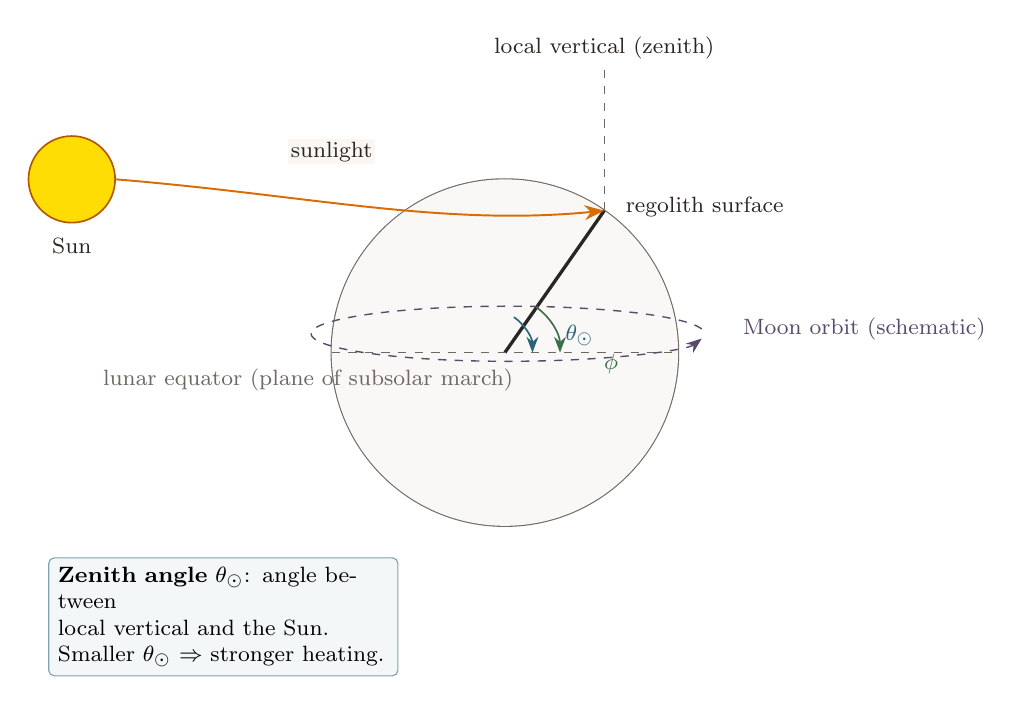
\begin{tikzpicture}[
  x=1cm, y=1cm,
  font=\small,
  sun/.style={circle, fill=yellow!80!orange, draw=orange!70!black, line width=0.6pt, minimum size=1.1cm},
  moon/.style={circle, fill=softgrey!40, draw=dim, line width=0.8pt},
  ray/.style={-{Stealth[length=2.5mm]}, line width=0.7pt, color=orange!85!black},
  dashedline/.style={dashed, color=dim, line width=0.5pt},
  label/.style={font=\footnotesize, text=char}
]

% Sun
\node[sun] (sun) at (-5.5, 2.2) {};
\node[label, below=2pt of sun] {Sun};

% Moon (cross-section)
\draw[moon] (0,0) circle (2.2);
\fill[softgrey!25] (0,0) circle (2.2);

% Local horizontal at site (latitude phi)
\coordinate (C) at (0,0);
\coordinate (S) at ({2.2*cos(55)},{2.2*sin(55)});  % site on surface, phi ~ 35 deg from equator visually
\draw[line width=1.2pt, color=char] (C) -- (S);
\node[label, anchor=west] at ($(S)+(0.15,0.05)$) {regolith surface};

% Vertical at site (local zenith)
\draw[dashedline] (S) -- ++(0, 1.8) node[above, label] {local vertical (zenith)};

% Sun ray to site
\draw[ray] (sun.east) .. controls (-2.5, 2.0) and (-0.8, 1.6) .. (S);
\node[label, fill=paper, inner sep=1pt] at (-2.2, 2.55) {sunlight};

% Solar zenith angle theta
\draw[{Stealth[length=2mm]}-, line width=0.6pt, color=teal] (0.35, 0) arc (0:55:0.55);
\node[label, text=teal] at (0.95, 0.22) {$\theta_\odot$};

% Latitude phi from equator
\draw[dashedline] (-2.2, 0) -- (2.2, 0);
\draw[{Stealth[length=2mm]}-, line width=0.6pt, color=forest] (0.7, 0) arc (0:55:0.7);
\node[label, text=forest] at (1.35, -0.15) {$\phi$};

% Equator hint
\node[label, text=dim] at (-2.5, -0.35) {lunar equator (plane of subsolar march)};

% Orbit hint
\draw[-{Stealth[length=2mm]}, line width=0.5pt, color=plum, dashed]
  (2.5, 0.3) arc (10:350:2.5 and 0.35);
\node[label, text=plum, anchor=west] at (2.9, 0.3) {Moon orbit (schematic)};

% Annotation box
\node[draw=teal!60, fill=teal!5, rounded corners=2pt, align=left, font=\footnotesize,
      text width=4.2cm, anchor=north west] at (-5.8, -2.6) {
  \textbf{Zenith angle} $\theta_\odot$: angle between\\
  local vertical and the Sun.\\
  Smaller $\theta_\odot$ $\Rightarrow$ stronger heating.
};

\end{tikzpicture}
\caption{\textbf{Sun--Moon--surface geometry.} At a site at latitude $\phi$, the
  Sun is not overhead at ``noon'' unless $\phi=0$. The \textbf{solar zenith angle}
  $\theta_\odot$ sets how much solar power hits each square metre of horizontal
  ground (cosine law). The retrieval uses an idealised cycle
  $\cos\theta_\odot(t)=\cos\phi\cos(2\pi t/P)$; full SPICE ephemeris lives in
  \file{lunar/ephem.py} but is not required for the \Kdstar{} fit.}
\label{fig:sun-moon-geometry}
\end{figure}

\subsubsection{From geometry to insolation: the cosine law}

The solar constant $S_0 \approx \SI{1361}{W/m^2}$ is the flux in a beam
perpendicular to the Sun. On a \textbf{horizontal} patch of ground, only the
component normal to the beam counts:
\begin{equation}
  F_\odot(t) = \max\!\bigl(0,\; S_0 \cos\theta_\odot(t)\bigr).
  \label{eq:insolation-teach}
\end{equation}
When the Sun is low ($\theta_\odot$ large), $\cos\theta_\odot$ is small and
heating is weak. At night, $\cos\theta_\odot < 0$ and the $\max(0,\cdot)$ clips
insolation to zero.

\paragraph{Idealised synodic model used in production.}
For each site latitude $\phi$,
\begin{equation}
  \cos\theta_\odot(t) = \cos\phi \,\cos\!\left(\frac{2\pi t}{P}\right),
  \label{eq:cos-zenith-ideal}
\end{equation}
with $P = \code{T\_LUNAR}$. This is the same formula as in the manuscript
(Eq.~\eqref{eq:insolation-teach}). It assumes:
\begin{itemize}[leftmargin=1.4em,itemsep=1pt]
  \item smooth variation over one lunation (no libration jitter at the hour scale),
  \item no solar \textbf{declination} tilt ($\pm 1.5^\circ$ neglected),
  \item no orbital \textbf{eccentricity} changing $S_0$ ($<0.1\%$ effect on cycle mean).
\end{itemize}
Those corrections matter for \emph{phase-resolved} work; this project compares
\textbf{time-mean} temperatures over a stability window, so the simplified cycle is
adequate (see manuscript \S``Surface solar geometry'').


% ---- Figure: insolation over one lunation --------------------------------
\begin{figure}[htbp]
\centering
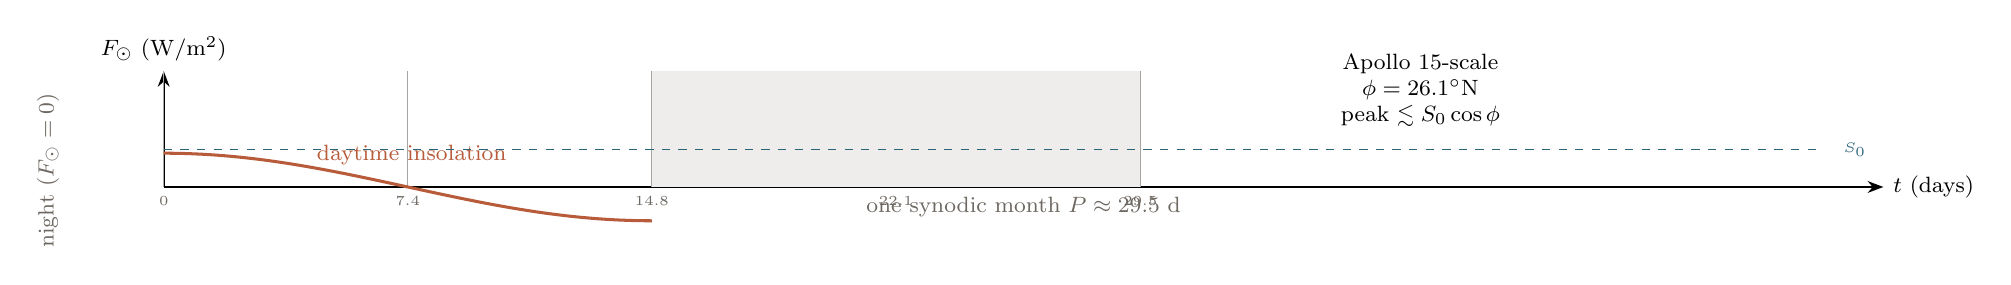
\begin{tikzpicture}[x=0.42cm, y=0.00035cm, font=\small]
  % Axes
  \draw[-{Stealth}, line width=0.6pt] (0,0) -- (52,0) node[right, font=\footnotesize] {$t$ (days)};
  \draw[-{Stealth}, line width=0.6pt] (0,0) -- (0,4200)
    node[above, font=\footnotesize] {$F_\odot$ (\si{W/m^2})};
  \draw[color=dim!60, line width=0.3pt] (0,0) -- (0,4200);
  \draw[color=dim!60, line width=0.3pt] (7.38,0) -- (7.38,4200);
  \draw[color=dim!60, line width=0.3pt] (14.76,0) -- (14.76,4200);
  \draw[color=dim!60, line width=0.3pt] (22.14,0) -- (22.14,4200);
  \draw[color=dim!60, line width=0.3pt] (29.53,0) -- (29.53,4200);
  \node[below, font=\tiny, text=dim] at (0,0) {0};
  \node[below, font=\tiny, text=dim] at (7.38,0) {7.4};
  \node[below, font=\tiny, text=dim] at (14.76,0) {14.8};
  \node[below, font=\tiny, text=dim] at (22.14,0) {22.1};
  \node[below, font=\tiny, text=dim] at (29.53,0) {29.5};
  \node[below, font=\footnotesize, text=dim] at (26, -28)
    {one synodic month $P \approx 29.5$~d};

  % cos curve for phi = 26 deg (peak ~ 1223 W/m2); day half only
  \draw[line width=1.1pt, color=coral, domain=0:14.76, samples=80]
    plot (\x, {1361*0.899*cos(360*\x/29.53)});

  % Night shading
  \fill[dim!12] (14.76,0) rectangle (29.53,4200);

  \node[font=\footnotesize, text=dim, rotate=90] at (-3.5, 600) {night ($F_\odot=0$)};
  \node[font=\footnotesize, text=coral] at (7.5, 1150) {daytime insolation};
  \node[font=\footnotesize, align=center] at (38, 3500) {Apollo~15-scale\\$\phi=26.1^\circ$N\\peak $\lesssim S_0\cos\phi$};

  % S0 reference
  \draw[dashed, color=teal, line width=0.6pt] (0,1361) -- (50,1361);
  \node[font=\tiny, text=teal, anchor=west] at (50.5, 1361) {$S_0$};

\end{tikzpicture}
\caption{\textbf{Idealised insolation} $F_\odot(t)$ for northern mid-latitude
  ($\cos\phi \approx 0.90$). Sunlit half of the lunation: flux follows a cosine;
  night: clipped to zero. Peak is below $S_0$ because the Sun never reaches the
  zenith at $\phi > 0$. Code: \code{insol = S0 * cos\_lat * np.maximum(0, np.cos(phase))}
  in \file{retrieve\_kd.py}.}
\label{fig:insolation-lunation}
\end{figure}

\subsubsection{Top boundary: surface energy balance (control volume)}

Take a thin control volume \emph{at} the surface --- the top face sees space, the
bottom face touches the first regolith cell. In steady balance at each instant,
Eq.~\eqref{eq:bc-top-teach} applies (derived in \autoref{sec:bc-full}), with
insolation written explicitly as $F_\odot(t)$ instead of $S(t)$:
\[
  (1-A)\,F_\odot(t) \;=\; \varepsilon\sigma T_s(t)^4 \;+\; q_{\mathrm{cond}}(t).
\]
Here $q_{\mathrm{cond}} = -K\,\partial T/\partial z\big|_{z=0}$ is the downward
conductive flux (positive when heat enters the ground).

% ---- Figure: surface energy balance --------------------------------------
\begin{figure}[htbp]
\centering
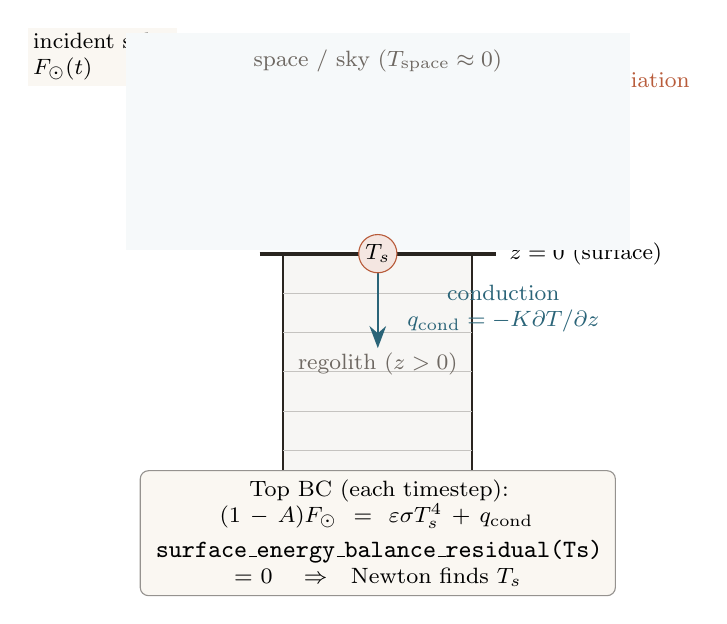
\begin{tikzpicture}[
  x=1cm, y=1cm, font=\small,
  arr/.style={-{Stealth[length=2.8mm]}, line width=0.85pt},
  thinarr/.style={-{Stealth[length=2mm]}, line width=0.6pt}
]

% Regolith column
\fill[softgrey!35] (-1.2, -2.8) rectangle (1.2, 0);
\draw[line width=0.8pt, color=char] (-1.2, -2.8) rectangle (1.2, 0);
\foreach \y in {-0.5,-1.0,-1.5,-2.0,-2.5} {
  \draw[dim!40, line width=0.3pt] (-1.2,\y) -- (1.2,\y);
}
\node[font=\footnotesize, text=dim] at (0, -1.4) {regolith ($z>0$)};

% Surface line
\draw[line width=1.4pt, color=char] (-1.5, 0) -- (1.5, 0);
\node[anchor=west, font=\footnotesize] at (1.55, 0) {$z=0$ (surface)};

% Sun / insolation from upper left
\draw[arr, color=orange!85!black] (-2.8, 2.2) -- (-0.3, 0.35);
\node[align=left, font=\footnotesize, fill=paper, inner sep=2pt] at (-3.5, 2.5) {
  incident solar\\$F_\odot(t)$
};
\draw[thinarr, color=orange!60!black] (-1.0, 1.5) -- (-0.2, 0.25);
\node[align=left, font=\footnotesize, text=orange!70!black] at (-2.2, 1.0) {
  absorbed\\$(1-A)F_\odot$
};

% Reflected (small arrow back)
\draw[thinarr, color=dim, dashed] (-0.1, 0.2) -- (-1.2, 1.0);
\node[font=\tiny, text=dim] at (-1.5, 1.15) {reflected $AF_\odot$};

% Outgoing IR upward
\draw[arr, color=coral] (0.2, 0.15) -- (0.2, 2.0);
\node[align=left, font=\footnotesize, text=coral, anchor=west] at (0.45, 2.0) {
  emitted thermal radiation\\$\varepsilon\sigma T_s^4$
};

% Conduction downward
\draw[arr, color=teal] (0, -0.05) -- (0, -1.2);
\node[align=center, font=\footnotesize, text=teal, anchor=west] at (0.25, -0.7) {
  conduction\\$q_{\mathrm{cond}}=-K\partial T/\partial z$
};

% Sky
\fill[teal!4] (-3.2, 0.05) rectangle (3.2, 2.8);
\node[font=\footnotesize, text=dim] at (0, 2.45) {space / sky ($T_{\mathrm{space}}\approx 0$)};

% Ts label
\node[circle, fill=coral!15, draw=coral, inner sep=1pt, font=\footnotesize\bfseries] at (0, 0) {$T_s$};

% Balance equation box
\node[draw=char!50, fill=paper, rounded corners=3pt, align=center, font=\footnotesize,
      text width=5.8cm] at (0, -3.55) {
  Top BC (each timestep): \quad
  $(1-A)F_\odot = \varepsilon\sigma T_s^4 + q_{\mathrm{cond}}$\\[3pt]
  \code{surface\_energy\_balance\_residual(Ts)} = 0
  \quad$\Rightarrow$\quad Newton finds $T_s$
};

\end{tikzpicture}
\caption{\textbf{Top boundary control volume.} Absorbed sunlight (after albedo $A$)
  must equal the sum of infrared emission and heat conducted into the regolith.
  $T_s$ is not stored as a fixed number --- it is \textbf{solved} each hour so the
  balance holds. This is what \code{\_solve\_surface\_newton} does in
  \file{solver.py}.}
\label{fig:surface-energy-balance}
\end{figure}

\begin{analogy}
The surface is like a pan on a stove that also glows in the dark. Sunlight pours
in (when it's day), the pan radiates heat to the cold kitchen (space), and the
handle (regolith) conducts heat downward. At every instant the pan's top temperature
adjusts until those three flows balance.
\end{analogy}

\subsubsection{How orbital forcing connects to the heat equation}

The chain from orbit to interior is:
\begin{center}
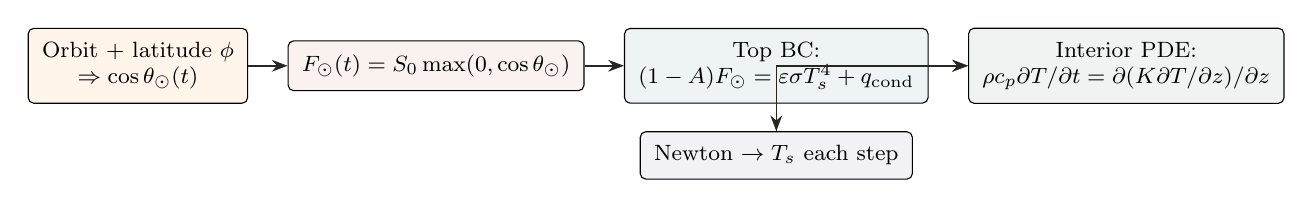
\begin{tikzpicture}[
  node distance=0.35cm and 0.5cm,
  box/.style={draw, rounded corners=2pt, fill=paper, align=center,
              font=\footnotesize, inner sep=5pt, minimum width=2.6cm},
  arr/.style={-{Stealth[length=2mm]}, line width=0.55pt, color=char}
]
\node[box, fill=orange!8] (orbit) {Orbit + latitude $\phi$\\$\Rightarrow\cos\theta_\odot(t)$};
\node[box, fill=coral!8, right=of orbit] (insol) {$F_\odot(t)=S_0\max(0,\cos\theta_\odot)$};
\node[box, fill=teal!8, right=of insol] (bc) {Top BC:\\$(1-A)F_\odot=\varepsilon\sigma T_s^4+q_{\mathrm{cond}}$};
\node[box, fill=forest!8, right=of bc] (pde) {Interior PDE:\\$\rho c_p\partial T/\partial t=\partial(K\partial T/\partial z)/\partial z$};
\node[box, fill=plum!8, below=of bc] (newton) {Newton $\to T_s$ each step};
\draw[arr] (orbit) -- (insol);
\draw[arr] (insol) -- (bc);
\draw[arr] (bc) -- (pde);
\draw[arr] (bc) -- (newton);
\draw[arr] (newton) |- (pde);
\end{tikzpicture}
\end{center}

Insolation is \textbf{prescribed} (known input from orbit model). Skin temperature
$T_s$ is \textbf{unknown} until the top BC is satisfied. Once $T_s$ is known, it
feeds the first interior cell and Crank--Nicolson advances $T(z,t)$ for all deeper
layers.

\subsubsection{Bottom boundary (for completeness)}

\begin{figure}[htbp]
\centering
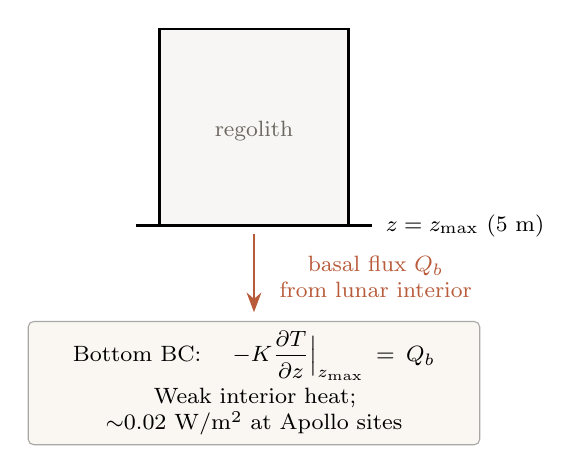
\begin{tikzpicture}[x=1cm, y=1cm, font=\small,
  arr/.style={-{Stealth[length=2.5mm]}, line width=0.75pt}]
\fill[softgrey!35] (-1.2, 0) rectangle (1.2, 2.5);
\draw[line width=0.8pt] (-1.2, 0) rectangle (1.2, 2.5);
\node[font=\footnotesize, text=dim] at (0, 1.2) {regolith};
\draw[line width=1.2pt] (-1.5, 0) -- (1.5, 0);
\node[anchor=west, font=\footnotesize] at (1.55, 0) {$z=z_{\mathrm{max}}$ (5~m)};
\draw[arr, color=coral] (0, -0.1) -- (0, -1.1);
\node[align=center, font=\footnotesize, text=coral, anchor=west] at (0.2, -0.65) {
  basal flux $Q_b$\\from lunar interior
};
\node[draw=char!40, fill=paper, rounded corners=2pt, font=\footnotesize, align=center,
      text width=5.5cm] at (0, -2.0) {
  Bottom BC: \quad $-K\dfrac{\partial T}{\partial z}\Big|_{z_{\mathrm{max}}} = Q_b$\\[2pt]
  Weak interior heat; ${\sim}0.02$~\si{W/m^2} at Apollo sites
};
\end{tikzpicture}
\caption{\textbf{Bottom boundary.} A small steady flux from the Moon's interior.
  No orbital variation --- only the top sees the Sun.}
\label{fig:bottom-bc}
\end{figure}

\begin{headsup}
\textbf{What is \emph{not} in the top BC.} No atmosphere, no wind, no latent heat
(evaporation), no ground heat storage in a separate surface layer. The model is
deliberately minimal: radiative balance + 1-D conduction. That matches airless-body
practice for metre-scale regolith (Hayne et al.\ 2017; Vasavada et al.\ 2012).
\end{headsup}

\subsubsection{Code map: from \code{insolation} to \code{\_step}}

\begin{table}[htbp]
\centering
\small
\begin{tabular}{@{}llp{6.2cm}@{}}
\toprule
Step & Function / variable & Role \\
\midrule
1 & \code{cos\_lat = np.cos(np.radians(lat))} & latitude factor \\
2 & \code{phase = 2*np.pi*t/T\_LUNAR} & lunation phase \\
3 & \code{insol = S0 * cos\_lat * max(0, cos(phase))} & build $F_\odot(t)$ \\
4 & \code{run\_with(..., insolation=insol)} & pass into solver \\
5 & \code{\_solve\_surface\_newton(T\_prev, insol\_k, ...)} & top BC $\to T_s$ \\
6 & \code{\_step(...)} & CN step for interior + bottom $Q_b$ \\
\bottomrule
\end{tabular}
\caption{End-to-end path for orbital forcing and boundary conditions in the retrieval pipeline.}
\label{tab:orbit-bc-code}
\end{table}

For full SPICE-based zenith angles (sub-solar latitude, libration, exact timestamps),
see \file{lunar/ephem.py}. The \Kdstar{} retrieval does not require that path because
it fits \emph{mean} temperatures, not diurnal phase.


\section{The numerical method, gently}
\label{sec:numerics}

The heat equation (\autoref{sec:heateq}) is a continuous statement about every
point and every instant. A computer can't handle ``infinitely many points.'' So
we \textbf{discretize}: chop space into finite slices and time into finite steps,
and turn the calculus into arithmetic the computer can repeat millions of times.

\subsection{Slicing the depth: why a \emph{geometric} grid}
\label{sec:grid}

We split the 5-metre soil column into many thin horizontal layers and track one
temperature per layer. The clever part: the layers are \textbf{not equally
thick}.
\begin{itemize}[leftmargin=1.4em,itemsep=3pt]
  \item Near the surface, temperature swings violently over a few centimetres
    (the skin). To capture that we need \textbf{very thin} layers
    (${\sim}\SI{2}{mm}$ at the top).
  \item Deep down, temperature barely changes over a whole metre. Thin layers
    there would just waste computer effort.
\end{itemize}
So each layer is made ${\sim}8\%$ thicker than the one above it. This is a
\textbf{geometric grid} (each step multiplied by a constant ratio).

\begin{figure}[h]
\centering
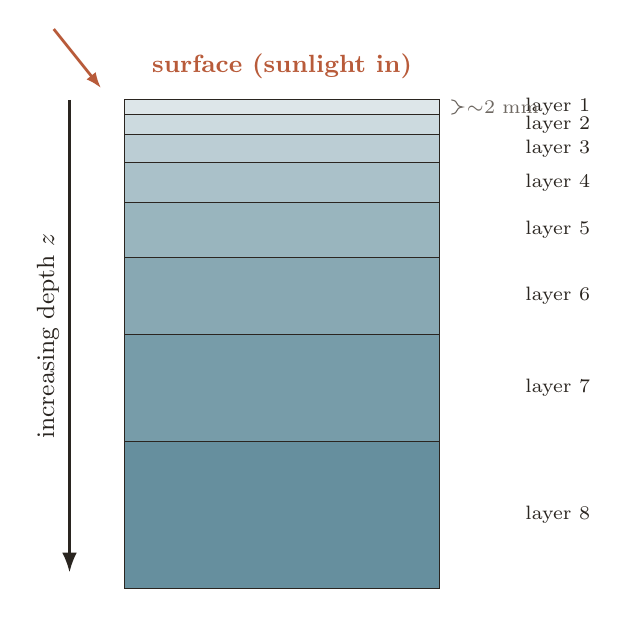
\begin{tikzpicture}[x=1cm,y=1cm]
  % geometric layer boundaries (exaggerated for clarity)
  \def\xL{0} \def\xR{4}
  \pgfmathsetmacro{\prev}{0}
  \foreach \i/\h in {1/0.18, 2/0.26, 3/0.36, 4/0.50, 5/0.70, 6/0.98, 7/1.36, 8/1.86} {
    \pgfmathsetmacro{\top}{\prev}
    \pgfmathsetmacro{\bot}{\prev+\h}
    \fill[teal!\the\numexpr8+\i*8\relax] (\xL,-\top) rectangle (\xR,-\bot);
    \draw[char,line width=0.4pt] (\xL,-\top) rectangle (\xR,-\bot);
    \node[char,font=\scriptsize] at (\xR+1.5,{-(\top+\bot)/2}) {layer \i};
    \global\let\prev\bot
  }
  % surface label + sun
  \node[coral,font=\bfseries\small,anchor=south] at (2,0.15) {surface (sunlight in)};
  \draw[-{Latex[length=2mm]},coral,line width=1pt] (-0.9,0.9) -- (-0.3,0.15);
  % depth arrow
  \draw[-{Latex[length=2.5mm]},char,line width=0.9pt] (-0.7,0) -- (-0.7,-6.0)
    node[midway,left,rotate=90,anchor=south,font=\small] {increasing depth $z$};
  % bracket on first thin layer
  \draw[decorate,decoration={brace,amplitude=4pt},dim]
    (\xR+0.15,0) -- (\xR+0.15,-0.18) node[midway,right,font=\scriptsize,xshift=2pt] {${\sim}2$ mm};
\end{tikzpicture}
\caption[The geometric depth grid]{The geometric depth grid (thicknesses
exaggerated). \textbf{What to notice:} slices are paper-thin at the top, where
the daily heat wave is sharp, and grow ${\sim}8\%$ thicker with each step
downward, so the deep, sleepy soil is covered cheaply. \textbf{Why it matters:}
this puts the computational effort exactly where the physics is fast-changing
--- like taking many photos per second of a sprint start but only one per minute
of a marathon's middle.}
\label{fig:grid}
\end{figure}

The grid docstring in \file{lunar/grid.py} puts it perfectly:

\begin{lstlisting}[language={},style=shellstyle,caption={From the \file{lunar/grid.py} docstring.}]
Near the surface, where temperature swings wildly between lunar day
and night, we use paper-thin slices (~2 mm) so we capture the fast
changes. Deeper down, where temperature barely moves, the slices get
gradually thicker (each ~8% thicker than the one above). This
"geometric" spacing puts the computational effort where the action is.
\end{lstlisting}

The grid is built by \code{make\_geometric\_grid}, configured in
\file{lunar/config.py}:

\begin{lstlisting}[caption={The production grid in \file{lunar/config.py}.}]
# --- depth grid (geometric) ---
GRID = dict(z_max=5.0, dz0=0.002, growth=0.08)
\end{lstlisting}

That reads: total depth \SI{5}{m}, top layer \SI{2}{mm} thick, each next layer
$8\%$ thicker (growth ratio 1.08). Uniform grids are \emph{deliberately
forbidden} in this project (the code even raises an error) because they
under-resolve the skin while wasting effort deep down.

\begin{headsup}
\file{lunar/constants.py} also defines \emph{fallback} grid defaults
(\code{Z\_MAX\_DEFAULT = 3.0}, \code{GROWTH\_DEFAULT = 0.15}). Those are only used
if someone calls \code{make\_geometric\_grid()} with no arguments. The real
science runs always pass \code{GRID} from \file{config.py} (\SI{5}{m} /
\SI{2}{mm} / 1.08), so the production grid is the \file{config.py} one. Don't be
confused by the two different numbers.
\end{headsup}

\subsection{Stepping through time: what a ``timestep'' is}
\label{sec:timestep}

We also chop \textbf{time} into steps. Here each step $\Delta t$ is \textbf{one
hour} (\code{DT\_STEP = 3600.0} seconds in \file{config.py}). Starting from the
temperatures right now, we apply the heat equation to compute the temperatures
one hour later, then repeat. One full lunar day (a ``lunation'') is
${\sim}29.5$ Earth days (\SI{2551443}{s}), so one simulated lunation is
\textbf{709 hourly samples} (\code{N\_t = int(T\_LUNAR / DT\_STEP) + 1} in
\code{run\_with}). The test suite samples more coarsely (2-hour steps) to keep
continuous-integration runs fast.

\begin{headsup}
\textbf{A handy units gotcha.} Watch out for the number 2551: it looks like a
timestep count but is really the lunation \emph{length} in thousands of seconds
(\SI{2551443}{s}). The number of hourly steps is \textbf{709}.
\end{headsup}

\subsection{Crank--Nicolson: a stable, accurate way to take a step}
\label{sec:cn}

There are simple ways to step a heat equation forward, but the na\"ive ones
either blow up (become numerically unstable) unless the timestep is
microscopically small, or they are inaccurate. \textbf{Crank--Nicolson} is the
standard professional choice. Intuition:
\begin{itemize}[leftmargin=1.4em,itemsep=3pt]
  \item An \textbf{explicit} step computes the future purely from the present.
    Cheap, but unstable for stiff problems like heat (it can oscillate and
    explode).
  \item An \textbf{implicit} step computes the future from the future (you solve
    a small system of equations). Stable, but slightly less accurate.
  \item \textbf{Crank--Nicolson averages the two} (``half now, half later,'' the
    $0.5$ factors you'll see in the code). The result is both \textbf{stable}
    \emph{and} \textbf{second-order accurate} in time. It is coded in
    \code{\_step} in \file{lunar/solver.py} (look for the \code{0.5 * alpha\_...}
    terms --- that $0.5$ \emph{is} the Crank--Nicolson averaging).
\end{itemize}

\begin{keyidea}
You don't need to derive it. Just know: Crank--Nicolson is the recipe that lets
us take comfortable one-hour steps without the simulation exploding.
\end{keyidea}

\subsection{The tridiagonal (Thomas) solver: the fast inner engine}
\label{sec:thomas}

An implicit / Crank--Nicolson step requires solving a system of linear
equations: ``find all the new-layer temperatures at once such that they are
mutually consistent.'' Normally solving $N$ equations in $N$ unknowns is slow
(cost grows like $N^3$). But here each layer only talks to its \textbf{immediate
neighbours above and below} --- so the system is \textbf{tridiagonal} (nonzero
only on the diagonal and the two adjacent diagonals).

For tridiagonal systems there is a famous shortcut, the \textbf{Thomas
algorithm}, that solves them in a single sweep down and a single sweep back up
--- cost grows only like $N$ (linear), which is as fast as it gets. It is
implemented in \code{\_thomas} in \file{lunar/solver.py}:

\begin{lstlisting}[caption={The Thomas tridiagonal solver, \file{lunar/solver.py}.}]
@njit(cache=True)
def _thomas(a, b, c, d):
    """Thomas algorithm for an (a, b, c) tridiagonal system A x = d."""
    n = b.size
    cp = np.empty(n); dp = np.empty(n); x = np.empty(n)
    cp[0] = c[0] / b[0]
    dp[0] = d[0] / b[0]
    for i in range(1, n):                 # forward sweep
        m = b[i] - a[i] * cp[i - 1]
        cp[i] = c[i] / m if i < n - 1 else 0.0
        dp[i] = (d[i] - a[i] * dp[i - 1]) / m
    x[n - 1] = dp[n - 1]
    for i in range(n - 2, -1, -1):        # back substitution
        x[i] = dp[i] - cp[i] * x[i + 1]
    return x
\end{lstlisting}

The \code{@njit} decorator is \textbf{Numba}, a tool that compiles this Python
down to machine code so it runs ${\sim}10$--$100\times$ faster (this inner loop
runs millions of times). If Numba isn't installed, the code falls back to plain
Python and still works --- see the \code{try/except} at the top of
\file{lunar/solver.py}. (\file{docs/} contains \file{NUMBA\_VS\_CPP\_JUSTIFICATION.md}
explaining why Numba was chosen over writing C++.)

\begin{figure}[h]
\centering
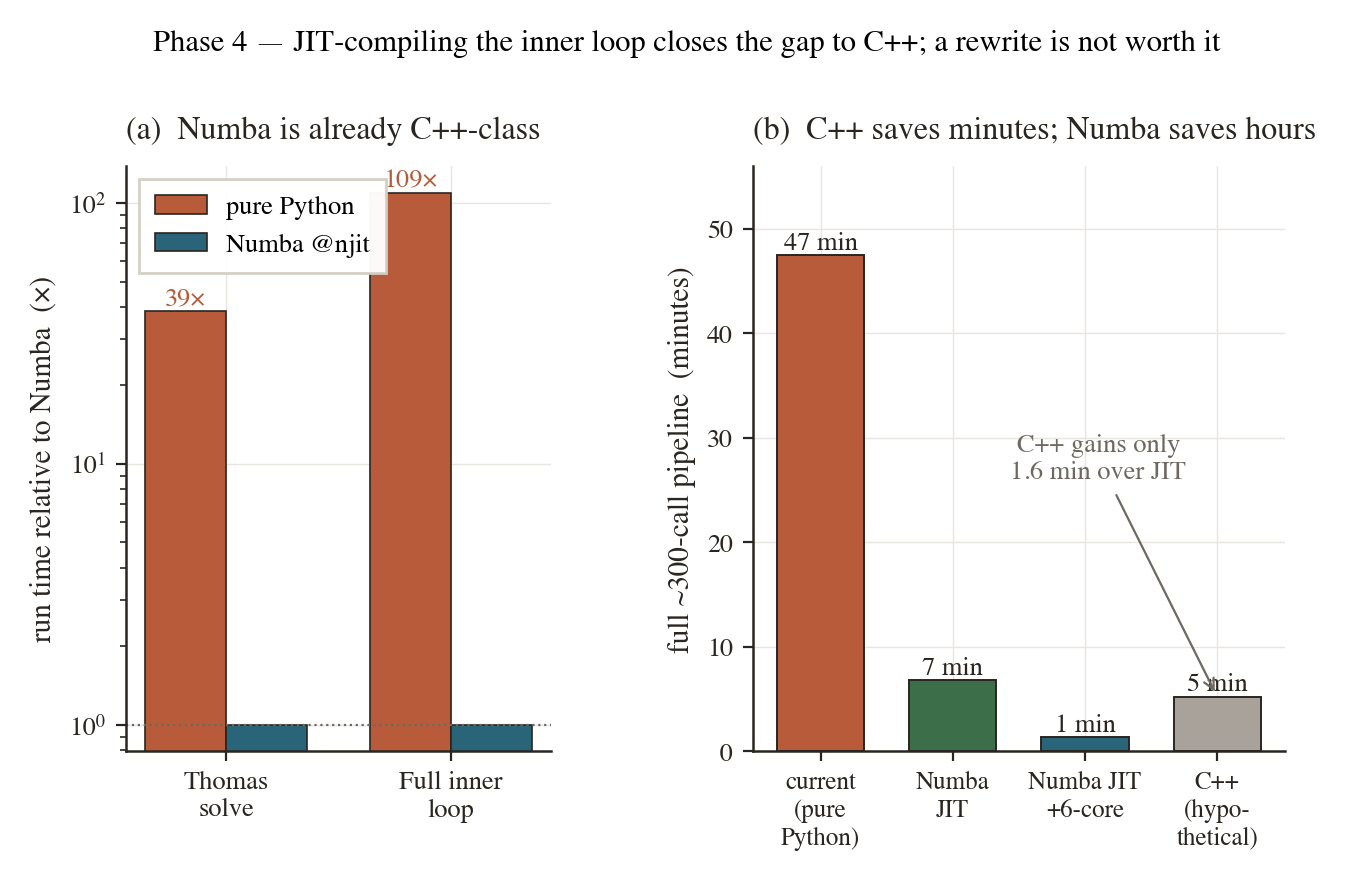
\includegraphics[width=0.82\textwidth]{fig_phase4_njit_vs_cpp.png}
\caption[Numba speed-up]{Why the \code{@njit} compiler matters: a benchmark of
the solver's inner loop. \textbf{What to notice:} compiling the hot Python loop
with Numba closes almost all of the gap to hand-written C++, while keeping the
code in one readable language. \textbf{Why it matters:} the retrieval runs the
solver hundreds of times, so this speed-up is what makes the whole study
practical on a laptop.}
\label{fig:njit}
\end{figure}

One more detail: conductivity between two adjacent layers uses the
\textbf{harmonic mean} (\code{\_face\_harmonic\_mean}), not the simple average.
For heat flowing \emph{through} two materials in series (like the deep,
conductive layer feeding the fluffy, insulating layer above), the harmonic mean
is the physically correct combination --- the poor conductor dominates, just as
the narrowest pipe dominates a series of pipes.

\subsection{Newton's method for the non-linear surface}
\label{sec:newton}

Remember the surface radiates as $T_s^4$ (\autoref{sec:boundaries}). That fourth
power makes the surface energy-balance equation \textbf{non-linear} --- you can't
just solve for $T_s$ algebraically. Instead we use \textbf{Newton's method}, the
classic ``guess, check the error, slide toward the answer, repeat'' root-finder:
\begin{enumerate}[leftmargin=1.5em,itemsep=2pt]
  \item Guess a surface temperature $T_s$.
  \item Compute the \textbf{residual} $R(T_s)$ --- how badly the energy balance
    fails (absorbed $-$ radiated $-$ conducted;
    \code{surface\_energy\_balance\_residual}).
  \item Use the slope $\mathrm{d}R/\mathrm{d}T_s$ to jump to a better guess.
  \item Repeat until $R$ is ${\sim}0$ (a few iterations).
\end{enumerate}
This is \code{\_solve\_surface\_newton} in \file{lunar/solver.py}. The code notes
the derivative is always negative, which guarantees Newton converges from any
positive starting temperature. So at \textbf{every hourly step}, the solver does
a tiny Newton solve to pin the surface temperature, then a Thomas sweep to update
the whole column. That's the complete inner loop.

\section{The Anchor Point Method (the centerpiece)}
\label{sec:anchor}

This is the \textbf{centerpiece} of the project --- the clever idea that makes
the whole thing fast \emph{and} trustworthy. It lives in
\file{lunar/equilibrium.py}. Read that file's docstring; it's excellent. This
section builds on it.

\subsection{The problem: the deep Moon settles agonizingly slowly}

We want the \textbf{periodic steady state}: the repeating day-after-day
temperature pattern the soil settles into after a long time, when every lunar day
looks like the last. To get there the obvious approach is ``spin-up'' --- just
press play and simulate many lunar days until things stop changing.

The catch: the \textbf{deep} column relaxes on the \emph{diffusion timescale of
the whole 5-metre column}, which is roughly \textbf{1000 lunar days}. Simulating
1000 lunations per run, for the ${\sim}300$ runs the retrieval needs, is
hopeless.

Worse, if you stop early (say after 30 lunations), the deep temperature still
\textbf{secretly remembers your starting guess}. And the deep temperature is
exactly what the Apollo sensors measure. So your ``measurement'' of \Kd{} would
be contaminated by an arbitrary guess you typed in. This was a real, critical bug
caught in the project's own audit --- \textbf{flag F1} in
\file{docs/FLAG\_REPORT.md}. The original code used hard-coded starting
temperatures (\SI{250}{\kelvin} for A15, \SI{255}{\kelvin} for A17), and a
$\pm\SI{5}{\kelvin}$ change in that guess swung the retrieved \Kdstar{} by a
factor of ${\sim}6$ --- \emph{larger than the very inter-site contrast the paper
reports!} That had to be fixed before any result could be believed.

\subsection{The key insight: two clocks}
\label{sec:twoclocks}

The fix comes from realizing the soil has \textbf{two very different ``clocks'':}
\begin{itemize}[leftmargin=1.4em,itemsep=3pt]
  \item \textbf{The shallow skin (top ${\sim}$half metre) is FAST.} It settles
    into its repeating day/night rhythm within a handful of lunar days, because
    it is thin and driven hard by the surface.
  \item \textbf{The deep column is SLOW} to settle by brute force --- \emph{but}
    in steady state it must obey one dead-simple rule: the same steady interior
    heat \Qb{} flows through every layer. That single rule,
    $\mathrm{d}\langle T\rangle/\mathrm{d}z = Q_b/K$, \textbf{fixes the entire
    deep temperature shape instantly} --- no waiting required. ($\langle T\rangle$
    means the cycle-averaged temperature; the angle brackets denote ``average
    over one day.'')
\end{itemize}
So instead of waiting 1000 lunations for the deep column, we \textbf{calculate}
it from the steady-flux rule, and only ever simulate the fast skin.

\subsubsection{Where $\mathrm{d}\langle T\rangle/\mathrm{d}z = Q_b/K$ comes from}

Same physics as \autoref{sec:boundaries} (geothermal gradient), now as the
anchor shortcut:
\begin{enumerate}[leftmargin=1.5em,itemsep=2pt]
  \item Time-average the heat equation over one lunation.
  \item In periodic steady state: $\partial\langle T\rangle/\partial t=0$.
  \item Equation collapses to $\partial[K\,\partial\langle T\rangle/\partial z]/\partial z=0$.
  \item So $K\,\mathrm{d}\langle T\rangle/\mathrm{d}z=Q_b$ everywhere below the skin.
  \item Integrate downward from the anchor: \code{\_reconstruct\_subskin} in
    \file{lunar/equilibrium.py}.
\end{enumerate}

\subsubsection{The rectified flux $u_{\mathrm{rect}}$}

Inside the skin, $\langle K\,\partial T/\partial z\rangle \neq K(\langle T\rangle)\,
\mathrm{d}\langle T\rangle/\mathrm{d}z$. The extra \textbf{rectification} term
$u_{\mathrm{rect}}$ is measured from the resolved cycle (\code{\_rectified\_flux})
and subtracted:
$\mathrm{d}\langle T\rangle/\mathrm{d}z = (Q_b - u_{\mathrm{rect}})/K$.
Negligible below \SI{1}{m}; a few percent near \SI{0.3}{m}--\SI{0.5}{m} --- why
the anchor sits at \SI{0.55}{m}.

\begin{figure}[h]
\centering
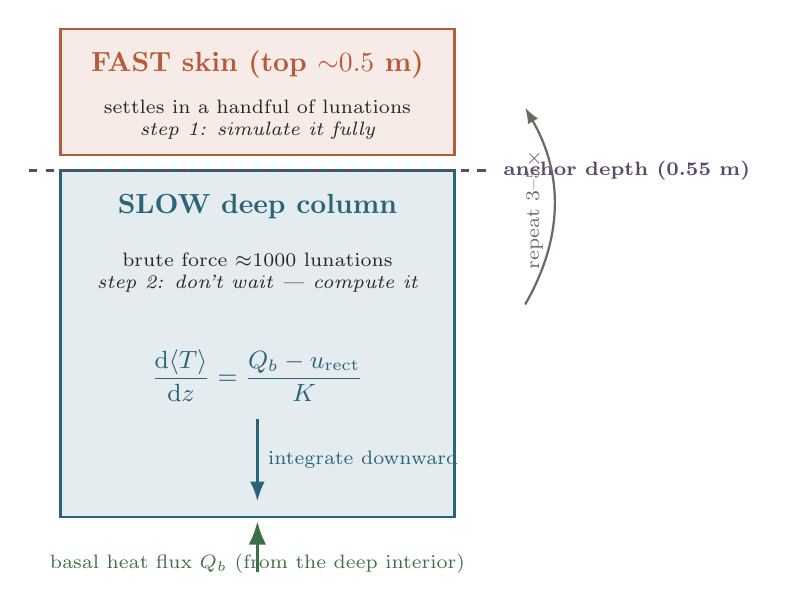
\begin{tikzpicture}[x=1cm,y=1cm,font=\small]
  % skin box
  \fill[coral!12] (0,0) rectangle (5,-1.6);
  \draw[coral,line width=0.9pt] (0,0) rectangle (5,-1.6);
  \node[coral,font=\bfseries] at (2.5,-0.45) {FAST skin (top ${\sim}0.5$ m)};
  \node[char,font=\scriptsize,align=center] at (2.5,-1.15)
    {settles in a handful of lunations\\ {\itshape step 1: simulate it fully}};
  % deep box
  \fill[teal!12] (0,-1.8) rectangle (5,-6.2);
  \draw[teal,line width=0.9pt] (0,-1.8) rectangle (5,-6.2);
  \node[teal,font=\bfseries] at (2.5,-2.25) {SLOW deep column};
  \node[char,font=\scriptsize,align=center] at (2.5,-3.1)
    {brute force ${\approx}1000$ lunations\\ {\itshape step 2: don't wait --- compute it}};
  % flux rule
  \node[teal,font=\small] at (2.5,-4.4) {$\dfrac{\mathrm{d}\langle T\rangle}{\mathrm{d}z}=\dfrac{Q_b-u_{\mathrm{rect}}}{K}$};
  \draw[-{Latex[length=2.5mm]},teal,line width=1pt] (2.5,-4.95) -- (2.5,-6.0)
     node[midway,right,font=\scriptsize] {integrate downward};
  % anchor
  \draw[dashed,plum,line width=1pt] (-0.4,-1.8) -- (5.4,-1.8);
  \node[plum,font=\bfseries\scriptsize,anchor=west] at (5.5,-1.8) {anchor depth (0.55 m)};
  % basal flux arrow
  \draw[-{Latex[length=3mm]},forest,line width=1.2pt] (2.5,-6.9) -- (2.5,-6.25)
     node[below,font=\scriptsize,yshift=-8pt,forest] {basal heat flux $Q_b$ (from the deep interior)};
  % outer loop arrows on the side
  \draw[-{Latex[length=2mm]},dim,line width=0.8pt]
     (5.9,-3.5) to[out=60,in=-60] (5.9,-1.0);
  \node[dim,font=\scriptsize,rotate=90,anchor=south] at (6.25,-2.3) {repeat 3--5$\times$};
\end{tikzpicture}
\caption[The two-clock Anchor Point Method]{The Anchor Point Method as ``two
clocks.'' \textbf{What to notice:} the fast skin is simulated in full (step~1);
the slow deep column is \emph{reconstructed} from the steady-flux rule
(step~2) rather than waited out, anchored to the cycle-mean temperature read at
$0.55$~m. The two steps are repeated a few times until they agree.
\textbf{Why it matters:} this turns an impossible ${\sim}1000$-lunation wait into
a handful of cheap iterations, while removing the starting-guess bias.}
\label{fig:twoclocks}
\end{figure}

\subsection{The method: alternate ``settle the skin'' and ``rebuild the deep''}

The algorithm (the ``outer iteration'') alternates two cheap steps until they
agree:
\begin{enumerate}[leftmargin=1.5em,itemsep=4pt]
  \item \textbf{Settle the skin.} Run the full solver for just a few lunar days
    (\code{n\_inner = 12}) starting from the current profile. This locks the fast
    skin into rhythm against the current deep column.
  \item \textbf{Rebuild the deep.} Read the cycle-mean temperature at one trusted
    \textbf{anchor depth} just below the skin (\code{z\_anchor = 0.55} m), then
    integrate the steady-flux rule
    $\mathrm{d}\langle T\rangle/\mathrm{d}z = (Q_b - u_{\mathrm{rect}})/K$
    \emph{downward} from there to reconstruct the entire deep profile exactly.
\end{enumerate}
Repeat steps 1--2 a few times (typically 3--5). The result ``locks on'' to the
true periodic steady state. The actual loop is \code{solve\_periodic\_equilibrium}
in \file{lunar/equilibrium.py}; the deep rebuild is \code{\_reconstruct\_subskin}.

Two refinements worth knowing:
\begin{itemize}[leftmargin=1.4em,itemsep=3pt]
  \item \textbf{$u_{\mathrm{rect}}$ --- the rectified flux.} Inside the skin, the
    daily wobble plus the fact that conductivity depends on temperature creates a
    small extra \emph{day--night-averaged} heat term (an ``eddy'' or
    ``rectification'' term). The code measures it exactly from the resolved cycle
    (\code{\_rectified\_flux}) and subtracts it, so the deep rebuild stays
    accurate. It is negligible below ${\sim}1$~m but matters a few percent right
    at the anchor --- which is precisely why the anchor is placed at
    $0.55$~m, \emph{below} the worst of it.
  \item \textbf{Two-stage anchor schedule.} The code first anchors high
    ($0.25$~m, relaxes fast) to cheaply kill most of the starting-guess error,
    then drops to $0.55$~m for the accurate finish. See the \code{stages} tuple
    in \code{solve\_periodic\_equilibrium}.
\end{itemize}

\subsection{Why it's both fast \emph{and} unbiased}

\begin{itemize}[leftmargin=1.4em,itemsep=3pt]
  \item \textbf{Fast:} it only ever simulates the quick skin (a few lunations per
    outer step, ${\sim}36$--$60$ lunations total) instead of ${\sim}1000$.
    Comparable cost to the old broken spin-up, but correct.
  \item \textbf{Unbiased (this is the crucial part):} the final answer \textbf{no
    longer depends on the starting guess}. The skin is forced periodic by step~1;
    the deep is forced to satisfy steady flux by step~2. The only fixed point of
    that two-step map is the \emph{true} equilibrium. The starting guess just
    seeds the first iterate and gets erased.
\end{itemize}

This is \textbf{certified, not assumed.} The regression test
\code{tests/test\_equilibrium.py::test\_guess\_independence} literally runs the
solver from two different starting guesses (\SI{242}{\kelvin} and
\SI{258}{\kelvin}) and asserts the converged profiles agree:

\begin{lstlisting}[caption={The guess-independence regression test.}]
def test_guess_independence():
    """Converged profiles from 242 K and 258 K guesses must agree."""
    grid, t, insol, k_func, cp_func = _setup()
    profiles = []
    for guess in (242.0, 258.0):
        eq = solve_periodic_equilibrium(
            grid=grid, t=t, insolation=insol, albedo=0.131,
            emissivity=0.95, Q_b=0.021, K_func=k_func, cp_func=cp_func,
            T_guess=guess)
        assert eq.converged
        profiles.append(eq.T_mean)
    assert np.max(np.abs(profiles[0] - profiles[1])) < 0.1
\end{lstlisting}

In the full production setting the guess-dependence is $\le \SI{0.023}{\kelvin}$
(vs the old \SI{1.6}{}--\SI{4.5}{\kelvin}). That is what ``F1 RESOLVED'' at the
top of \file{docs/FLAG\_REPORT.md} means, and it's why the retrieved \Kdstar{}
values can be trusted.

\subsection{``Flux closure'' --- how the code proves it worked}

How do you know the deep profile really satisfies steady heat flow? You check
whether the cycle-mean conductive flux equals \Qb{} at every depth. The maximum
relative deviation is the \textbf{flux closure} number (\code{flux\_closure} in
\code{EquilibriumResult}). The retrieval warns if closure is worse than $3\%$. It
is deliberately measured \textbf{below the diurnal skin} (where the rule actually
applies and where every Apollo sensor sits), not at the noisy surface. The test
\code{test\_flux\_closure} checks this. The
\code{make\_equilibrium\_certification.py} figure script visualizes the whole
certification.

\section{The \texorpdfstring{\Kd}{Kd} retrieval and uncertainty analysis}
\label{sec:retrieval}

Now we connect the simulator to the real Apollo data and extract \Kd. The driver
is \file{scripts/pipeline/retrieve\_kd.py}.

\subsection{The data: turning raw HFE records into ``equilibrium temperatures''}
\label{sec:data}

The bundled Apollo data lives in \file{data/apollo/depth/} as \file{.tab} text
files (one per mission per probe, e.g.\ \file{a15p1\_depth.tab}). Each row is a
timestamp, a temperature, a sensor name, and the sensor's depth in cm. The loader
is \code{load\_apollo\_hfe\_depth} (\file{lunar/validation.py}).

But the raw record drifts for years after the probes were emplaced (the drilling
disturbed the soil, which slowly re-equilibrated). We only want the final
\textbf{settled} temperature of each sensor. \code{find\_stable\_window}
(\file{lunar/apollo\_helpers.py}) scans the late part of each sensor's record and
picks the earliest window where the temperature has gone \textbf{flat} (trend
slope below \SI{0.08}{K/year}), then averages it. That average is the sensor's
\textbf{equilibrium temperature $T_{\mathrm{eq}}$}. \code{extract\_sensor\_stability}
does this for every sensor and returns depths $+$ $T_{\mathrm{eq}}$ values.

Crucially, only sensors \textbf{deeper than \code{MIN\_DEPTH\_CM = 80 cm}} are
used for the fit (the \code{deep\_mask}). Shallower sensors are contaminated by
the borestem (the hardware sticking up) and by the daily skin, so they are
excluded \emph{a priori}.

\subsection{The retrieval: sweep \texorpdfstring{\Kd}{Kd}, minimize RMSE}
\label{sec:sweep}

The core idea is a \textbf{sweep} (\code{run\_kd\_sweep\_extended}):
\begin{enumerate}[leftmargin=1.5em,itemsep=3pt]
  \item Pick a grid of candidate \Kd{} values (e.g.\ 28 values from 1 to
    \SI{15}{mW} for A15; see \code{KD\_GRIDS} in \file{config.py}).
  \item For each candidate \Kd{}, run the equilibrium solver (\code{run\_with},
    which calls \code{solve\_periodic\_equilibrium}) to get a predicted
    temperature-vs-depth profile.
  \item Read the model temperature at each real sensor depth and subtract the
    measured $T_{\mathrm{eq}}$. That difference is the \textbf{residual}.
  \item Combine the residuals into one number, the \textbf{RMSE}.
\end{enumerate}

\begin{plainenglish}
\textbf{RMSE $=$ Root Mean Square Error.} It is the standard ``how far off, on
average'' score: square every residual (so positives and negatives don't cancel
and big misses count extra), average them, take the square root. Smaller $=$
better fit. Units are kelvin here:
\[
  \mathrm{RMSE}(K_d) = \sqrt{\frac{1}{N}\sum_{i=1}^{N}
    \bigl[\,T_{\mathrm{model}}(z_i; K_d) - T_{\mathrm{eq},i}\,\bigr]^2}.
\]
\end{plainenglish}

The best-fit \Kdstar{} is the value that \textbf{minimizes} RMSE. The code even
fits a little parabola through the three points around the minimum to find the
bottom precisely (\code{kd\_star\_from\_residuals}). That's the whole retrieval:
\emph{slide the one knob \Kd{} until the model temperatures best match the
measured ones.}

\begin{figure}[h]
\centering
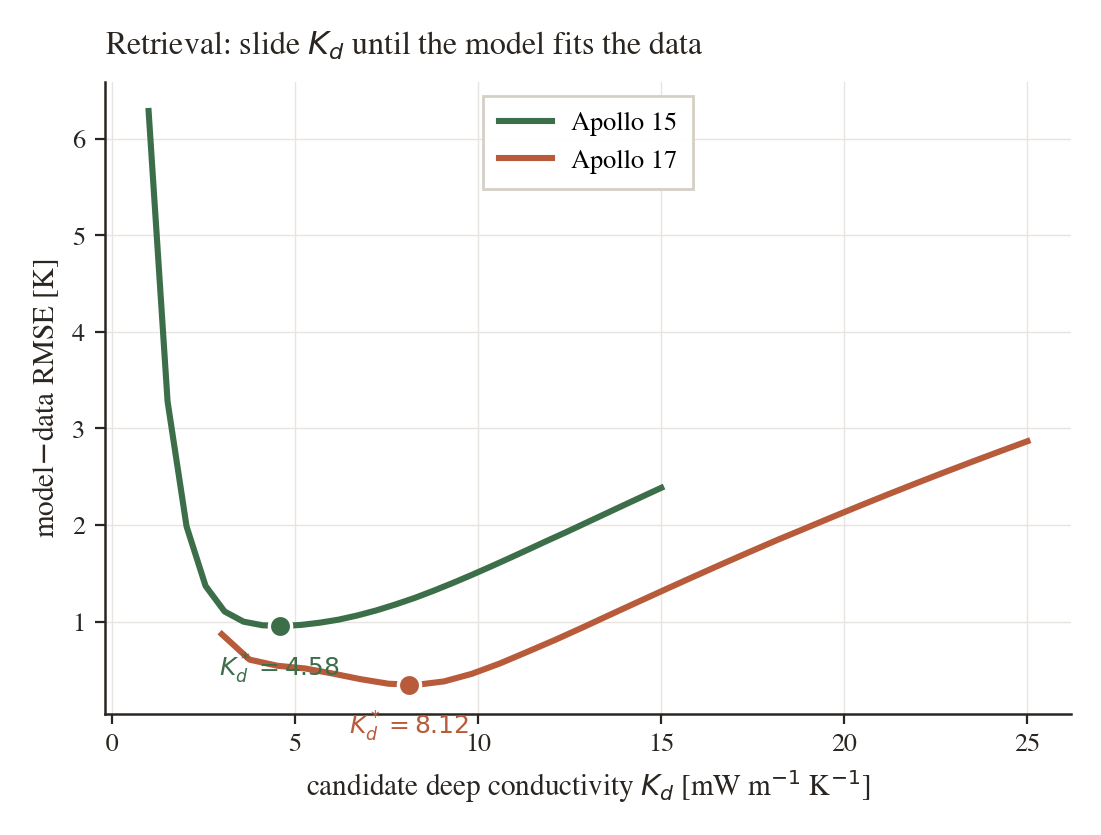
\includegraphics[width=0.80\textwidth]{fig_kd_retrieval.png}
\caption[The \Kd\ retrieval as an RMSE sweep]{The retrieval curve, computed from
the committed results. For each candidate deep conductivity \Kd{} we run the
simulator and score how far its temperatures land from the Apollo measurements
(RMSE). \textbf{What to notice:} each site's curve is a clean valley; its lowest
point is the retrieved \Kdstar{} (filled marker) --- \num{4.58}~\mwmk{} for
Apollo~15 and \num{8.12}~\mwmk{} for Apollo~17. \textbf{Why it matters:} the two
valleys sit at clearly different places, which is the visual heart of the
``the sites differ'' result.}
\label{fig:retrieval}
\end{figure}

Result: A15 lands at \Kdstar{}~${\approx}\num{4.58}$, A17 at
${\approx}\num{8.12}$~\mwmk{}, and switching to per-site values roughly
\textbf{halves} the Apollo-17 mismatch versus the old global \Kd{}~$=\num{3.4}$.

\subsection{Uncertainty: the bootstrap}
\label{sec:bootstrap}

A single best-fit number isn't science without an error bar. How sure are we? The
biggest uncertainty is that the \textbf{sensor depths themselves} are only known
to about $\pm\SI{2.5}{cm}$ (Nagihara~2018). The repo propagates this with a
\textbf{bootstrap} (\code{bootstrap\_kd\_with\_depth\_uncertainty}):
\begin{itemize}[leftmargin=1.4em,itemsep=3pt]
  \item Repeat 1500 times: randomly \textbf{resample} the sensors (draw with
    replacement) \emph{and} \textbf{jitter} each depth by a random
    $\pm\SI{2.5}{cm}$ wiggle, then re-find \Kdstar{}.
  \item You end up with 1500 slightly different \Kdstar{} values --- a whole
    distribution.
  \item The middle $95\%$ of that distribution is the \textbf{95\% confidence
    interval} (the $+1.33/-0.28$ style error bars).
\end{itemize}

\begin{analogy}
A bootstrap is just ``shake the inputs within their uncertainty, many times, and
watch how much the answer wobbles.'' The wobble \emph{is} the error bar. (The
bootstrap reuses cached solver outputs, so it is pure fast statistics --- no new
physics runs. It is ${\sim}65\%$ of the pipeline's runtime purely because of the
1500 repeats.)
\end{analogy}

\begin{figure}[h]
\centering

\includegraphics[width=0.92\textwidth]{fig_bootstrap.png}
\caption[Bootstrap distributions of the retrieved \Kdstar]{The bootstrap
distributions of \Kdstar{} for both sites. Each histogram is the spread of
answers you get when the sensor depths are jittered within their
$\pm\SI{2.5}{cm}$ uncertainty and the sensors are resampled, 1500 times. Dashed
lines mark the medians; shaded bands mark the 95\% confidence intervals.
\textbf{What to notice:} the two clouds barely overlap. \textbf{Why it matters:}
that separation is the quantitative statement that Apollo~17 conducts heat better
than Apollo~15 --- the contrast's confidence interval excludes zero
($p\approx0.01$).}
\label{fig:bootstrap}
\end{figure}

\subsection{Inter-site contrast and the \texorpdfstring{\Kd--\Qb}{Kd-Qb} degeneracy}
\label{sec:degeneracy}

The headline scientific claim is the \textbf{contrast}: A17~$-$~A15
${\approx}\num{3.3}$~\mwmk{}. Because we have a bootstrap distribution for
\emph{each} site, we can subtract them sample-by-sample to get a distribution for
the \textbf{difference}, and check whether it excludes zero. It does, at the
published heat fluxes: 95\% CI ${\approx}[0.4, 4.6]$, $p\approx0.01$
(\code{contrast\_bootstrap} in the results JSON).

The big caveat the paper is honest about: deep temperature depends on the
\textbf{ratio} $Q_b/K_d$, so \Kd{} and the basal flux \Qb{} are partly
\textbf{degenerate} --- if you assumed a different \Qb{}, you would retrieve a
different \Kd{}. That is why every result is stated \emph{``conditional on the
published basal heat fluxes.''} Propagating the full uncertainty in \Qb{} dilutes
the significance (the ordering probability drops to ${\sim}83\%$).

\begin{keyidea}
The honest summary: the sites differ in the combination $T(z)$ they produce;
attributing that purely to conductivity rather than basal flux rests on the
published \Qb{} values.
\end{keyidea}

Several auxiliary scripts probe robustness (held-out tests, model selection,
borestem cut, an independent Bayesian/MCMC cross-check) --- see
\autoref{sec:codetour}.

\subsection{The optional bedrock toggle (for future ice work)}
\label{sec:bedrock}

Recently added: an \textbf{optional bedrock layer} (\code{with\_bedrock} in
\file{lunar/properties.py}, configured by \code{BEDROCK} in
\file{lunar/config.py}). The standard model treats the Moon as fluffy regolith
all the way down. In reality, below ${\sim}\SI{10}{m}$ there is solid rock, which
conducts far better. \code{with\_bedrock} wraps any conductivity model so that
below \code{z\_bedrock} (\SI{10}{m}) the conductivity ramps smoothly (via a
\code{tanh}) up to a rock value (\code{K\_rock = 2.0}).

It is \textbf{OFF by default} and \textbf{does not change the published
retrieval} --- every Apollo sensor is at $\le\SI{2.4}{m}$, far above the
\SI{10}{m} transition, where enabling bedrock shifts temperatures by only
${\sim}\SI{0.05}{\kelvin}$. The tests \file{tests/test\_bedrock.py} lock in both
guarantees (off by default; sensor-depth temperatures unchanged). It exists for
\textbf{future deep-profile / ice-stability studies}, where the temperature far
below the regolith \emph{does} matter.

\section{Code tour: every file, in plain terms}
\label{sec:codetour}

A file-by-file map. Two layers: the \textbf{\file{lunar/} package} is the
reusable engine (all the physics and config); the \textbf{\file{scripts/}} are
thin command-line drivers that call the engine and write results/figures. There
is exactly one definition of everything --- config never gets copy-pasted.

\subsection{The \file{lunar/} package (the engine)}

\begin{longtable}{@{}p{0.30\textwidth}p{0.62\textwidth}@{}}
\toprule
\textbf{File} & \textbf{What it does, in plain terms} \\
\midrule
\endhead
\file{\_\_init\_\_.py} & Marks the folder as a package; sets the version. Nothing to study. \\
\file{constants.py} & The \textbf{physical numbers}: solar constant, Stefan--Boltzmann, regolith $K_s$/$K_d$/$H$/$\chi$, density / specific-heat coefficients, basal fluxes. Every value is cited to a paper. Project rule: no unsourced numbers. \\
\file{config.py} & The \textbf{settings menu / single source of truth}: the two-site table (\code{SITES}), the depth grid (\code{GRID}), the Hayne bundle (\code{HAYNE}), equilibrium-solver knobs, the \Kd{} sweep grids, the bedrock toggle. Change ``what the experiment is'' here. \\
\file{grid.py} & Builds the \textbf{geometric depth grid} (\code{make\_geometric\_grid} $\to$ a \code{DepthGrid} of layer faces, centres, thicknesses). \autoref{sec:grid}. \\
\file{properties.py} & The \textbf{soil property formulas}: conductivity (\code{conductivity\_hayne}, \code{conductivity\_martinez}, \code{conductivity\_icy}), density (\code{density\_hayne}), specific heat (\code{specific\_heat}), and the optional \code{with\_bedrock} wrapper. \autoref{sec:properties}--\ref{sec:conductivity}. \\
\file{solver.py} & The \textbf{heat-equation engine}: one Crank--Nicolson step (\code{\_step}), the tridiagonal \code{\_thomas} solver, harmonic-mean faces, the Newton surface solve (\code{\_solve\_surface\_newton}), the driver \code{solve\_pixel}, and the analytical wave used for testing. \autoref{sec:numerics}. \\
\file{equilibrium.py} & The \textbf{Anchor Point Method}: \code{solve\_periodic\_equilibrium} plus helpers (\code{\_rectified\_flux}, \code{\_reconstruct\_subskin}, \code{\_diurnal\_skin\_index}, \code{\_mean\_flux\_closure}). Returns an \code{EquilibriumResult}. \autoref{sec:anchor}. \textbf{Read this docstring.} \\
\file{validation.py} & Loads the bundled \textbf{Apollo HFE} \file{.tab} data into numpy arrays (\code{load\_apollo\_hfe\_depth}). \\
\file{apollo\_helpers.py} & Turns raw HFE records into per-sensor \textbf{equilibrium temperatures}: \code{find\_stable\_window} (detect the settled tail) and \code{extract\_sensor\_stability}. \autoref{sec:data}. \\
\file{ephem.py} & A \textbf{correct SPICE/DE440 solar-position} helper (sun elevation $\to$ insolation). \emph{Note:} the \Kd{} pipeline uses the simpler idealized cosine forcing, not this. \\
\file{diviner.py} & Helpers for \textbf{Diviner} orbital surface-temperature data, used for the surface-temperature ``closure'' cross-check. \\
\file{plotting/style.py} & Shared \textbf{figure styling} (JGR:Planets sizes, colour palette, layout helpers). Importing it gives every figure a consistent look. \\
\file{\_bootstrap.py} & Small \textbf{environment bootstrap} so standalone scripts can find the package and the data. Plumbing, not physics. \\
\bottomrule
\end{longtable}

\subsection{\file{scripts/pipeline/} (compute results \texorpdfstring{$\to$}{->} write \file{output/*.json})}

\begin{longtable}{@{}p{0.36\textwidth}p{0.56\textwidth}@{}}
\toprule
\textbf{File} & \textbf{What it produces} \\
\midrule
\endhead
\file{retrieve\_kd.py} & \textbf{The main event.} Loads HFE data, runs the \Kd{} sweep $+$ bootstrap $+$ joint $(K_d,H)$ grid $+$ held-out tests, writes \file{output/kd\_retrieval\_results.json} and the bootstrap/robustness/holdout figures. Start here. \\
\file{compute\_headline\_rmse.py} & The headline RMSE-vs-\Kd{} numbers (a second grid as a cross-check). \\
\file{compute\_borestem\_sensitivity.py} & How \Kdstar{} changes if you move the shallow-sensor cutoff (the borestem-contamination test). \\
\file{compute\_stability\_threshold\_sensitivity.py} & How results depend on the ``flatness'' threshold used to detect equilibrium windows. \\
\file{compute\_surface\_bias\_test.py} & Tests for systematic surface-temperature bias. \\
\file{compute\_uniform\_kd\_sensitivity.py} & What you'd get with a single uniform \Kd{} (the ``old way'') for comparison. \\
\file{compute\_fixed\_input\_sensitivities.py} & How \Kdstar{} responds to fixed inputs (albedo, $H$, etc.) --- feeds the error budget. \\
\file{compute\_model\_selection.py} & Compares competing conductivity models (AICc model selection). \\
\file{compute\_error\_budget.py} & Assembles the full systematic error budget (paper Table~4). \\
\file{bayesian\_crosscheck.py} & An independent \textbf{MCMC/Bayesian} retrieval as a cross-check on the bootstrap. \\
\file{compute\_diviner\_closure.py} & Checks the model's surface temperature against orbital \textbf{Diviner} data. \\
\bottomrule
\end{longtable}

\subsection{\file{scripts/figures/} and \file{scripts/analysis/}}

\begin{itemize}[leftmargin=1.4em,itemsep=3pt]
  \item \file{scripts/make\_all\_figures.py} --- runs \textbf{every} figure
    generator in order.
  \item \file{make\_letter\_figures.py}, \file{make\_results\_figures.py},
    \file{make\_intro\_figures.py} --- the paper's figures.
  \item \file{make\_equilibrium\_certification.py}, \file{make\_equilibrium\_demo.py},
    and the animation scripts --- visualize the Anchor Point Method (great for
    understanding \autoref{sec:anchor}).
  \item \file{make\_primer\_figures.py}, \file{make\_book\_figures.py},
    \file{make\_codeguide\_figures.py} --- teaching figures for the
    manuscript/guidebook.
  \item \file{scripts/analysis/phase2\_depth\_convergence.py} --- the standalone
    ``what happens deep down?'' diagnostic (\autoref{sec:skin}). A great first
    script to \emph{run and read} (see \autoref{fig:phase2}).
  \item \file{scripts/fetch\_diviner.py} --- one-time download of Diviner data
    (${\sim}310$~MB).
  \item \file{scripts/run\_all\_timed.py} --- runs the whole pipeline with timing.
\end{itemize}

\begin{figure}[h]
\centering
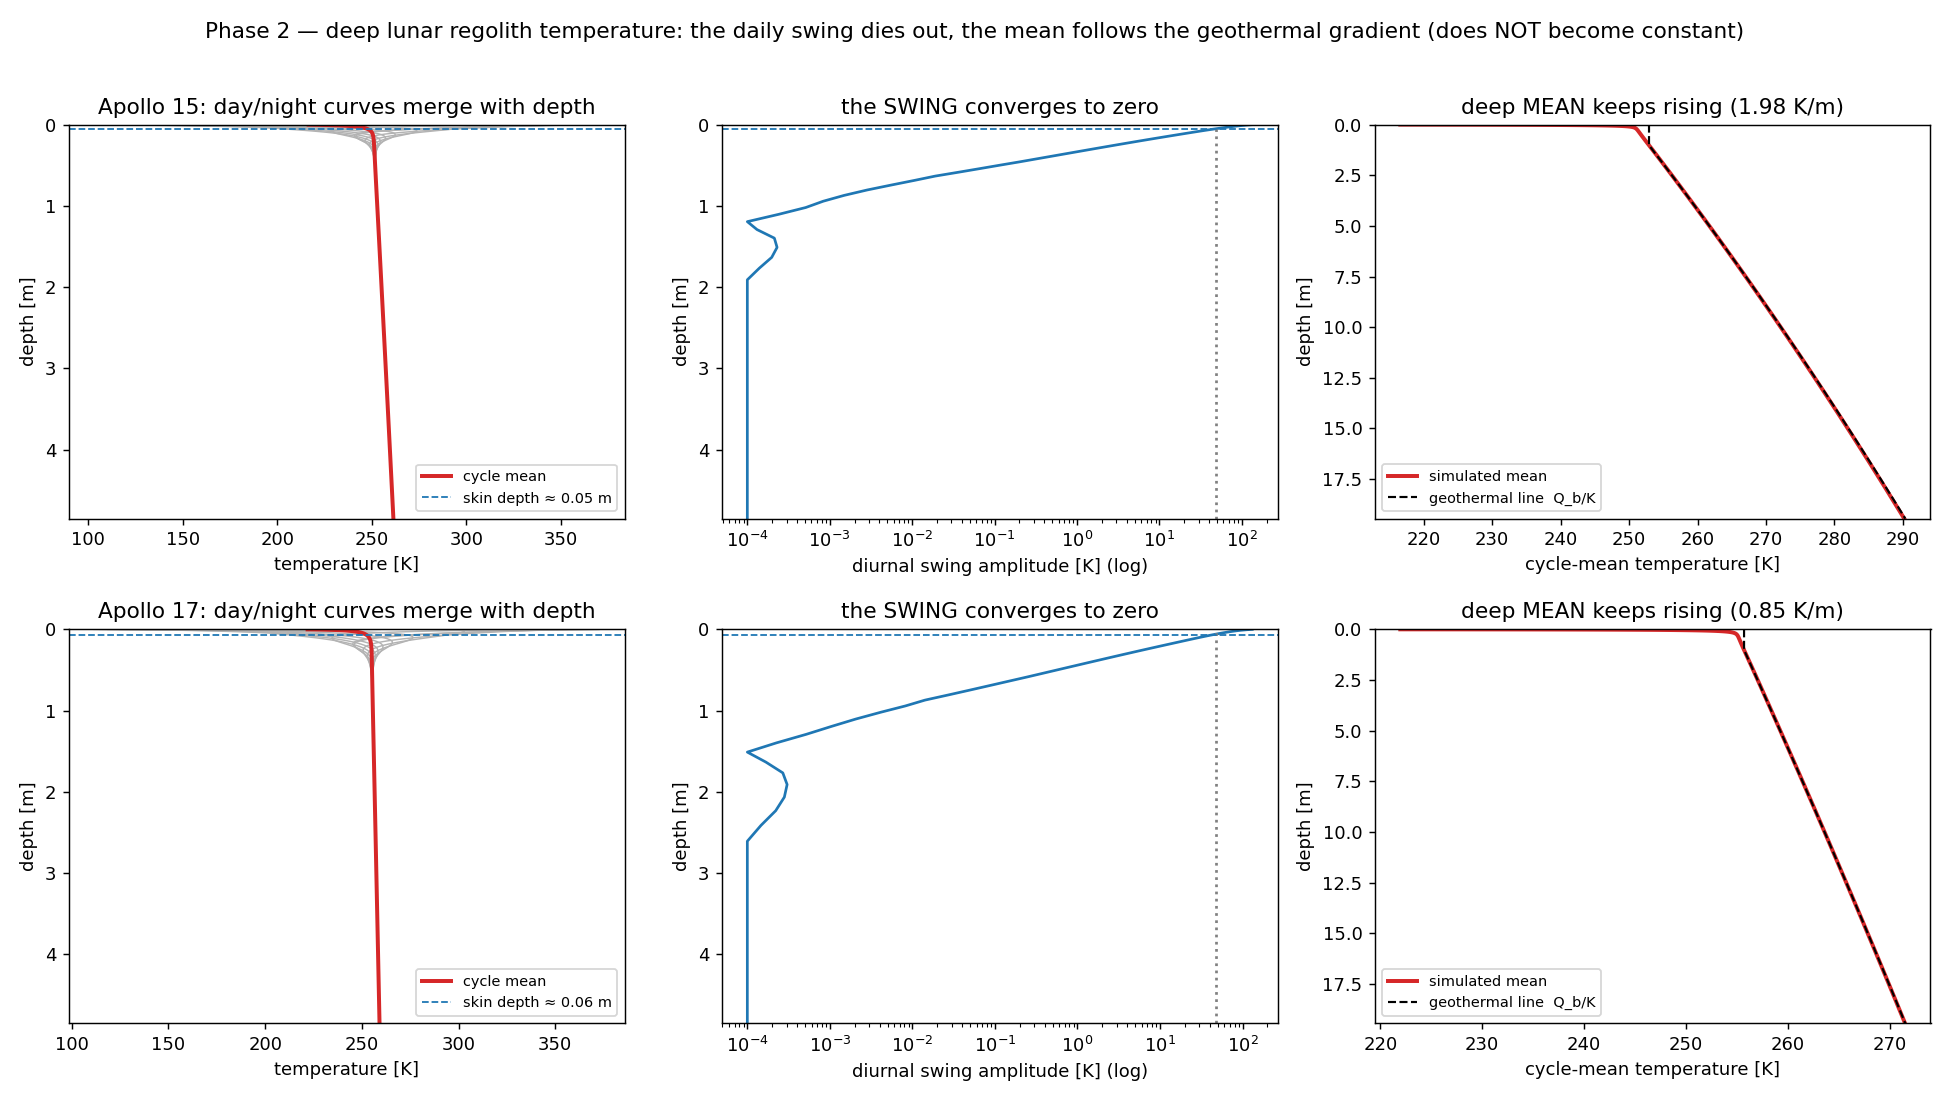
\includegraphics[width=0.96\textwidth]{fig_phase2_depth_convergence.png}
\caption[The phase-2 deep-temperature diagnostic]{The committed \code{phase2}
diagnostic, reproduced here for reference. \textbf{What to notice:} the left
panels show every-few-hours temperature curves merging onto a single line within
${\sim}1$~m; the middle panels show the swing damping toward zero; the right
panels show the cycle-mean continuing to rise along the geothermal line $Q_b/K$.
\textbf{Why it matters:} it is the same physics as
\autoref{fig:skin}--\ref{fig:meanprofile}, shown end to end on one sheet --- a
superb on-ramp to the project.}
\label{fig:phase2}
\end{figure}

\subsection{The end-to-end data flow}
\label{sec:dataflow}

\autoref{fig:dataflow} traces a single run from cited constants all the way to
the paper. Read it top-to-bottom: cited constants feed the config; the config
plus the property/grid modules feed the solver; the solver wrapped in the Anchor
Point Method produces a steady temperature profile; the retrieval slides \Kd{} to
match that profile to the processed Apollo data; the results become JSON, figures,
and ultimately the paper.

\begin{figure}[h]
\centering
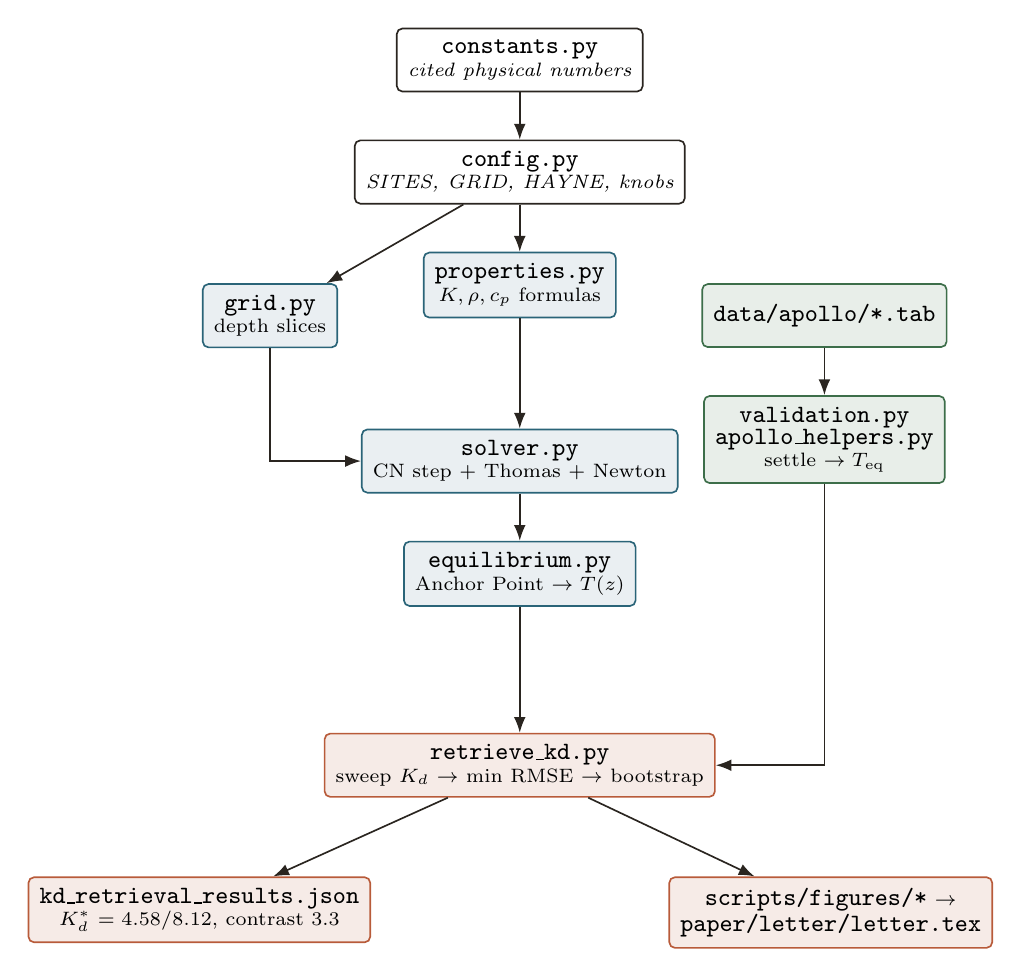
\begin{tikzpicture}[
   font=\scriptsize,
   node distance=6mm and 8mm,
   box/.style={draw=char,rounded corners=2pt,align=center,inner sep=4pt,
               minimum height=8mm,fill=white,line width=0.6pt},
   eng/.style={box,fill=teal!10,draw=teal},
   data/.style={box,fill=forest!12,draw=forest},
   outbox/.style={box,fill=coral!12,draw=coral},
   ar/.style={-{Latex[length=2mm]},char,line width=0.6pt}]

  \node[box] (const) {\file{constants.py}\\ \itshape cited physical numbers};
  \node[box,below=of const] (cfg) {\file{config.py}\\ \itshape SITES, GRID, HAYNE, knobs};

  \node[eng,below left=10mm and 2mm of cfg] (grid) {\file{grid.py}\\ depth slices};
  \node[eng,below=of cfg] (prop) {\file{properties.py}\\ $K,\rho,c_p$ formulas};
  \node[data,below right=10mm and 2mm of cfg] (tab) {\file{data/apollo/*.tab}};

  \node[eng,below=14mm of prop] (solver) {\file{solver.py}\\ CN step $+$ Thomas $+$ Newton};
  \node[data,below=of tab] (load) {\file{validation.py}\\ \file{apollo\_helpers.py}\\ settle $\to T_{\mathrm{eq}}$};

  \node[eng,below=of solver] (eq) {\file{equilibrium.py}\\ Anchor Point $\to T(z)$};

  \node[outbox,below=16mm of eq] (retr) {\file{retrieve\_kd.py}\\ sweep \Kd{} $\to$ min RMSE $\to$ bootstrap};

  \node[outbox,below left=10mm and -6mm of retr] (json) {\file{kd\_retrieval\_results.json}\\ \Kdstar{} $=4.58 / 8.12$, contrast 3.3};
  \node[outbox,below right=10mm and -6mm of retr] (paper) {\file{scripts/figures/*} $\to$\\ \file{paper/letter/letter.tex}};

  \draw[ar] (const) -- (cfg);
  \draw[ar] (cfg) -- (grid);
  \draw[ar] (cfg) -- (prop);
  \draw[ar] (grid) |- (solver);
  \draw[ar] (prop) -- (solver);
  \draw[ar] (tab) -- (load);
  \draw[ar] (solver) -- (eq);
  \draw[ar] (eq) -- (retr);
  \draw[ar] (load) |- (retr);
  \draw[ar] (retr) -- (json);
  \draw[ar] (retr) -- (paper);
\end{tikzpicture}
\caption[The end-to-end data flow]{The end-to-end pipeline. \textcolor{teal}{Teal}
boxes are the physics engine, \textcolor{forest}{green} boxes are the data path,
and \textcolor{coral}{coral} boxes are the outputs. \textbf{What to notice:}
everything funnels through one retrieval driver that compares simulated profiles
to processed Apollo temperatures. \textbf{Why it matters:} there is exactly one
path from a cited constant to a published number --- nothing is hand-edited along
the way.}
\label{fig:dataflow}
\end{figure}

\section{How to run it yourself}
\label{sec:running}

These commands are cross-checked against \file{docs/REPRODUCING.md} and the
\file{Makefile}. Run them from the repository root.

\subsection{One-time setup}

\begin{lstlisting}[style=shellstyle,caption={Create an isolated environment and install the package.}]
# 1. Create an isolated Python environment (so you don't clutter your system)
python3 -m venv .venv
source .venv/bin/activate        # Windows: .venv\Scripts\activate

# 2. Install the package + dev tools (pytest, jupyterlab, matplotlib, ...)
make install                     # same as: pip install -e ".[dev]"
\end{lstlisting}

A \textbf{virtual environment} (\code{venv}) is just a private sandbox of Python
packages for this project. \code{pip install -e .} installs the \code{lunar}
package in ``editable'' mode, meaning Python sees your local \file{lunar/} folder
directly --- edit a file and the change takes effect immediately.

\subsection{Run the tests first (always do this)}

\begin{lstlisting}[style=shellstyle]
python3 -m pytest -q
\end{lstlisting}

This runs the suite in \file{tests/} (grid, properties, solver, equilibrium,
bedrock, ephem, constants). They finish in under a minute and should
\textbf{all pass}. Reading a test is often the clearest example of how a function
is meant to be used.

\subsection{Verify the committed headline numbers (no computation needed)}

The canonical result ships in the repo, so you can check it instantly:

\begin{lstlisting}[caption={Verify the committed headline \Kdstar\ values.}]
import json, math
r = json.load(open('output/kd_retrieval_results.json'))
print('A15 K_d* =', r['A15']['kd_star'] * 1e3, 'mW/m/K')
print('A17 K_d* =', r['A17']['kd_star'] * 1e3, 'mW/m/K')
assert math.isclose(r['A15']['kd_star']*1e3, 4.58, abs_tol=0.01)
assert math.isclose(r['A17']['kd_star']*1e3, 8.12, abs_tol=0.01)
print('Headline values verified.')
\end{lstlisting}

\subsection{Reproduce the science (recompute from scratch)}

\begin{lstlisting}[style=shellstyle,caption={The one-word \file{Makefile} targets.}]
make help          # list every one-word command
make retrieve      # the core K_d retrieval + bootstrap (~5 min)
                   #   -> writes output/kd_retrieval_results.json
make aux           # all auxiliary sweeps, model selection, error budget, MCMC
make figures       # regenerate every figure
make paper         # compile the PDFs (needs a LaTeX install)
make all           # everything end-to-end
\end{lstlisting}

\code{make retrieve} is the one to run first --- it regenerates the headline JSON.
The slow auxiliary sweeps (\code{make aux}) are rarely needed because their
results are already committed.

\subsection{Run a single illuminating script}

To \emph{see} the deep-temperature physics (\autoref{sec:skin}) with your own
eyes:

\begin{lstlisting}[style=shellstyle]
python3 scripts/analysis/phase2_depth_convergence.py
\end{lstlisting}

It prints the skin depth, the deep gradient, and confirms the mean temperature
keeps rising along $Q_b/K$, then saves
\file{output/figures/fig\_phase2\_depth\_convergence.png}
(\autoref{fig:phase2}). Open that image. This is one of the best on-ramps to
understanding the project.

\begin{tryit}
Regenerate the five teaching figures in this very handbook. From the repository
root:
\begin{lstlisting}[style=shellstyle]
export MPLCONFIGDIR=/tmp/mpl
python3 docs/teaching/make_teaching_figures.py
\end{lstlisting}
This re-runs the certified equilibrium solver for both sites and re-reads the
committed results JSON, writing fresh PNG$+$PDF assets into
\file{docs/teaching/figures/}. Then rebuild this PDF with
\code{latexmk -pdf beginners\_guide.tex}.
\end{tryit}

\subsection{The notebooks (guided, in order)}

\begin{lstlisting}[style=shellstyle]
jupyter lab notebooks/
\end{lstlisting}

Run them in order: \code{00\_setup} (checks), \code{01\_methods} (figures $+$
parameter table), \code{02\_retrieval} (the \Kd{} retrieval $+$ bootstrap),
\code{03\_results}, \code{04\_discussion}, \code{05\_animations}. There's also
\code{equilibrium\_demo.ipynb}, a standalone demo that a brute-force
1000-lunation spin-up converges onto the fast Anchor Point solver --- a great way
to \emph{believe} \autoref{sec:anchor}.

\subsection{Where outputs land}

\begin{itemize}[leftmargin=1.4em,itemsep=2pt]
  \item \file{output/*.json} --- numerical results (the canonical
    \file{kd\_retrieval\_results.json} and the auxiliary JSONs).
  \item \file{output/figures/*.png} / \file{*.pdf} --- diagnostic and appendix
    figures.
  \item \file{paper/letter/figures/*.pdf} --- the paper's figures.
  \item \file{paper/letter/letter.pdf} --- the compiled manuscript.
\end{itemize}

\section{Glossary}
\label{sec:glossary}

Plain one-liners. Physics, then numerical, then code/project terms.

\subsection*{Physics}
\begin{description}[leftmargin=0pt,style=nextline,itemsep=2pt]
  \item[Regolith] The loose broken rock and dust covering the Moon; the ``soil.''
  \item[Temperature (K, kelvin)] How hot something is; a scale starting at
    absolute zero ($0$~K $=-273.15\,^\circ$C).
  \item[Heat flux] Rate of heat energy flow through a unit area (\unit{W/m^2}).
  \item[Conduction] Heat moving by direct contact, atom to atom.
  \item[Thermal conductivity $K$] How easily a material conducts heat
    (\unit{W.m^{-1}.K^{-1}}); high $=$ metal, low $=$ lunar dust.
  \item[\Kd] The \emph{deep} regolith conductivity; the quantity this project
    retrieves. \Kdstar{} is the best-fit value.
  \item[$K_s$] The \emph{surface} regolith conductivity (very low).
  \item[$H$ (scale height)] Sets how fast conductivity / density transition from
    surface to deep values (${\sim}\SI{6}{cm}$).
  \item[$\chi$ (chi, radiative coefficient)] Strength of the
    temperature-dependent radiative boost to conductivity (the $T^3$ term).
  \item[Density $\rho$ (rho)] Mass per unit volume (\unit{kg/m^3}).
  \item[Specific heat $c_p$] Energy to warm \SI{1}{kg} by \SI{1}{\kelvin}
    (\unit{J.kg^{-1}.K^{-1}}).
  \item[Thermal diffusivity $\alpha$] $K/(\rho c_p)$; how fast a temperature
    change spreads through a material.
  \item[Heat equation] The master PDE:
    $\rho c_p\,\partial T/\partial t = \partial/\partial z\,(K\,\partial T/\partial z)$.
    Derived step by step in \autoref{sec:heateq} from energy conservation in a
    thin soil slice plus Fourier's law.
  \item[Heat flux $q$] Thermal energy crossing a surface per second per m$^2$
    (\unit{W/m^2}); $q = -K\,\partial T/\partial z$.
  \item[Boundary condition] A rule at the domain edge that closes the PDE --- here,
    radiative balance at the surface and fixed geothermal flux $Q_b$ at depth.
  \item[Skin depth $\delta$] Depth over which a daily temperature wave fades to
    ${\sim}1/3$; a few cm on the Moon.
  \item[Insolation $S$] Incoming solar power per area at the surface
    (\unit{W/m^2}).
  \item[Albedo $A$] Fraction of sunlight reflected (${\approx}0.13$ here).
  \item[Emissivity $\varepsilon$] How efficiently a surface radiates heat
    (${\approx}0.95$).
  \item[Stefan--Boltzmann law] Radiated power $\propto T^4$; the $\sigma$ is its
    constant.
  \item[Geothermal / basal heat flux \Qb] Steady heat seeping up from the Moon's
    interior (${\sim}15$--$21$~\unit{mW/m^2}).
  \item[Periodic steady state / equilibrium] The repeating day-after-day
    temperature pattern reached after long settling.
  \item[Diurnal] Daily (here, one lunar day ${\approx}29.5$ Earth days, a
    ``lunation'').
\end{description}

\subsection*{Numerical}
\begin{description}[leftmargin=0pt,style=nextline,itemsep=2pt]
  \item[Discretize] Replace continuous space/time with finite slices/steps so a
    computer can solve it.
  \item[Grid] The set of depth slices; here \emph{geometric} (each slice
    ${\sim}8\%$ thicker than the one above).
  \item[Timestep $\Delta t$] The time jump per update (1 hour here).
  \item[Crank--Nicolson] A stable, accurate ``half-now, half-later''
    time-stepping scheme.
  \item[Tridiagonal system] A linear system where each unknown only couples to
    its two neighbours.
  \item[Thomas algorithm] The fast (linear-cost) solver for tridiagonal systems.
  \item[Harmonic mean] The correct way to average conductivity between two layers
    in series.
  \item[Newton's method] Iterative root-finder used for the non-linear surface
    temperature.
  \item[Residual] How badly an equation fails for a trial value (model $-$ data,
    or the energy-balance mismatch).
  \item[RMSE] Root-mean-square error; the average size of the model-vs-data
    mismatch (K).
  \item[Bootstrap] Estimate uncertainty by resampling/jittering inputs many times
    and watching the answer wobble.
  \item[Confidence interval (CI)] The range that contains the answer with stated
    probability (e.g.\ $95\%$).
  \item[Degeneracy] When two parameters trade off so only their combination is
    constrained (here \Kd{} and \Qb).
\end{description}

\subsection*{Code / project}
\begin{description}[leftmargin=0pt,style=nextline,itemsep=2pt]
  \item[Anchor Point Method] This project's fast, unbiased equilibrium solver
    (\autoref{sec:anchor}); the ``two clocks'' idea.
  \item[Flux closure] Diagnostic checking the mean conductive flux equals \Qb{}
    at depth (proof the solver converged).
  \item[$u_{\mathrm{rect}}$ (rectified flux)] Small day-night-averaged eddy heat
    term inside the skin, measured and subtracted.
  \item[Spin-up] Running many cycles to settle a simulation (the slow approach the
    Anchor Point Method replaces).
  \item[F1] The audit flag (in \file{docs/FLAG\_REPORT.md}) for the old
    starting-guess-bias bug that the Anchor Point Method fixed.
  \item[HFE] Apollo Heat-Flow Experiment (the buried thermometers).
  \item[Numba / \code{@njit}] A just-in-time compiler that speeds up the hot inner
    loops ${\sim}10$--$100\times$.
  \item[venv] An isolated Python environment for this project.
  \item[pytest] The tool that runs the test suite.
\end{description}

\section{A learning roadmap: what to study next}
\label{sec:roadmap}

A suggested order to go from ``I read this guide'' to ``I can change the code.''

\subsection*{Day 1 --- orient and run}
\begin{enumerate}[leftmargin=1.6em,itemsep=3pt]
  \item Re-read \autoref{sec:bigpicture} and
    \autoref{sec:physics}.1--\ref{sec:physics}.3 until ``heat $\ne$ temperature''
    and the heat equation feel natural.
  \item Do the setup (\autoref{sec:running}.1), run the tests
    (\autoref{sec:running}.2), verify the headline numbers
    (\autoref{sec:running}.3).
  \item Run \file{scripts/analysis/phase2\_depth\_convergence.py}
    (\autoref{sec:running}.5) and stare at the output figure while re-reading
    \autoref{sec:skin}. This makes skin depth and the geothermal gradient
    \emph{concrete}.
\end{enumerate}

\subsection*{Day 2 --- read the engine}
\begin{enumerate}[leftmargin=1.6em,itemsep=3pt,start=4]
  \item Read \file{lunar/constants.py} then \file{lunar/config.py} end to end ---
    they are short and define ``the experiment.''
  \item Read \file{lunar/properties.py} (\code{conductivity\_hayne},
    \code{density\_hayne}, \code{specific\_heat}) alongside
    \autoref{sec:properties}--\ref{sec:conductivity}.
  \item Read \file{lunar/grid.py} alongside \autoref{sec:grid}.
  \item Skim \file{lunar/solver.py}: focus on the \emph{docstring},
    \code{surface\_energy\_balance\_residual}, and \code{\_thomas}. Don't try to
    absorb every index in \code{\_step} yet.
\end{enumerate}

\subsection*{Day 3 --- the centerpiece}
\begin{enumerate}[leftmargin=1.6em,itemsep=3pt,start=8]
  \item Read the full docstring of \file{lunar/equilibrium.py} (it is a teaching
    text in itself), then \code{solve\_periodic\_equilibrium}, with
    \autoref{sec:anchor} open beside it.
  \item Read \file{tests/test\_equilibrium.py} --- the tests \emph{are} the
    precise statement of what ``correct'' means here.
  \item Optional: run \code{equilibrium\_demo.ipynb} to watch brute-force
    converge onto the fast method.
\end{enumerate}

\subsection*{Day 4 --- the science}
\begin{enumerate}[leftmargin=1.6em,itemsep=3pt,start=11]
  \item Read \file{scripts/pipeline/retrieve\_kd.py} top to bottom with
    \autoref{sec:retrieval} open. Follow one \Kd{} value through \code{run\_with}
    $\to$ \code{run\_kd\_sweep\_extended} $\to$ \code{kd\_star\_from\_residuals}.
  \item Read \file{lunar/apollo\_helpers.py} to see how raw data becomes
    $T_{\mathrm{eq}}$.
  \item Skim the paper abstract, plain-language summary, and \S2 (methods) in
    \file{paper/letter/letter.tex}.
\end{enumerate}

\subsection*{Then --- make a change (the real test of understanding)}
\begin{enumerate}[leftmargin=1.6em,itemsep=3pt,start=14]
  \item Try a tiny experiment: in a scratch script, call
    \code{run\_with(SITES['A15'], kd=...)} at a couple of \Kd{} values and print
    the temperature at $1.4$~m. Watch it move toward the data as \Kd{} approaches
    \num{4.58}.
  \item Read \file{docs/FLAG\_REPORT.md} to see how the project audits
    \emph{itself} --- this is how careful computational science is actually done.
\end{enumerate}

\subsection*{Deeper study, when ready}
\begin{itemize}[leftmargin=1.4em,itemsep=3pt]
  \item \textbf{Numerical methods:} the finite-volume method, implicit vs
    explicit schemes, stability (any intro numerical-PDE text).
  \item \textbf{Heat transfer:} Fourier's law and the 1-D heat equation (any
    intro heat-transfer text).
  \item \textbf{Python scientific stack:} NumPy basics (arrays, broadcasting,
    \code{np.interp}, \code{np.gradient}) --- used everywhere here.
  \item \textbf{Statistics:} the bootstrap and confidence intervals.
\end{itemize}

\begin{keyidea}
The single most effective habit: keep this guide open on one side and the actual
code file on the other. Every concept here points at a real function you can
open, run, and modify. Understanding grows fastest when the words and the code
are side by side.
\end{keyidea}


\end{document}
